% RESPAWN — English Grammar in Use, Units 1–17: mixed review (exercises)
% Compile with: pdflatex review-modules-1-17-exercises.tex  (run twice)

\documentclass[11pt,a4paper]{article}
\usepackage[T1]{fontenc}
\usepackage[utf8]{inputenc}
\usepackage{charter}
\usepackage[scaled=0.92]{helvet}
\usepackage{courier}
\usepackage[nointegrals]{wasysym}
\usepackage{amssymb}
\usepackage{pifont}
\usepackage[a4paper,left=17mm,right=17mm,top=21mm,bottom=19mm,headsep=6mm,footskip=10mm]{geometry}
\usepackage{xcolor}
\usepackage{tikz}
\usetikzlibrary{calc,positioning,arrows.meta,backgrounds,shapes.geometric,shapes.misc,fit,decorations.pathreplacing}
\usepackage[most]{tcolorbox}
\usepackage{enumitem}
\usepackage{multicol}
\usepackage{tabularx}
\usepackage{array}
\usepackage{booktabs}
\usepackage{colortbl}
\usepackage{fancyhdr}
\makeatletter
\newcommand{\needsp}[1]{\par\begingroup\setlength{\dimen@}{#1}\dimen@ii\pagegoal\advance\dimen@ii-\pagetotal
  \ifdim\dimen@>\dimen@ii\ifdim\dimen@ii>\z@\vfil\penalty-\@M\fi\fi\endgroup}
\makeatother
\raggedbottom
\usepackage{microtype}
\usepackage{etoolbox}
\usepackage{ragged2e}
\usepackage[hidelinks,pdftitle={Respawn - Units 1-17 review (exercises)},pdfauthor={FHX}]{hyperref}

% ---------- colours ----------
\definecolor{ink}{HTML}{1F2633}
\definecolor{inksoft}{HTML}{4A5466}
\definecolor{mute}{HTML}{8A93A3}
\definecolor{line}{HTML}{C3C9D4}
\definecolor{paper}{HTML}{F6F4EF}
\definecolor{accent}{HTML}{E8891D}
\definecolor{accentsoft}{HTML}{FDF0DF}
\definecolor{cDaily}{HTML}{2A9D8F}
\definecolor{cUni}{HTML}{3A6EA5}
\definecolor{cLab}{HTML}{C8553D}
\definecolor{cGame}{HTML}{7B5EA7}
\definecolor{cVault}{HTML}{B07D12}
\definecolor{good}{HTML}{2E8B57}
\definecolor{bad}{HTML}{C0392B}
\definecolor{dLotte}{HTML}{D1495B}
\definecolor{dWout}{HTML}{3A86C8}
\definecolor{dKai}{HTML}{2E9E6B}
\definecolor{dMira}{HTML}{B5509A}
\definecolor{dYou}{HTML}{E8891D}

% ---------- fonts ----------
\newcommand{\mdot}{\ensuremath{\cdot}}
\newcommand{\arr}{\ensuremath{\rightarrow}}
\newcommand{\hfont}{\fontfamily{pag}\selectfont}
\newcommand{\uifont}{\sffamily}
\setlength{\parindent}{0pt}
\setlength{\parskip}{4pt}
\linespread{1.04}
\setlist{nosep,leftmargin=*}
\renewcommand{\arraystretch}{1.15}

% ---------- small TikZ icons (drawn in mm, centred on 0,0) ----------
\tikzset{
  ic/.style={x=1mm,y=1mm,line width=0.5pt,line join=round,line cap=round},
  pics/house/.style={code={
    \draw (-1.1,-1.15) rectangle (1.1,0.3);
    \draw (-1.55,0.1) -- (0,1.35) -- (1.55,0.1);
    \fill (-0.35,-1.15) rectangle (0.35,-0.25);}},
  pics/cap/.style={code={
    \fill (-1.7,0.55) -- (0,1.35) -- (1.7,0.55) -- (0,-0.25) -- cycle;
    \fill (-0.95,0.05) -- (-0.95,-0.85) .. controls (0,-1.35) .. (0.95,-0.85) -- (0.95,0.05) -- (0,-0.4) -- cycle;
    \draw (1.35,0.62) -- (1.35,-0.75);}},
  pics/flask/.style={code={
    \draw (-0.42,1.35) -- (-0.42,0.35) -- (-1.3,-1.2) -- (1.3,-1.2) -- (0.42,0.35) -- (0.42,1.35);
    \draw (-0.65,1.35) -- (0.65,1.35);
    \fill (-0.86,-0.42) -- (-1.3,-1.2) -- (1.3,-1.2) -- (0.86,-0.42) -- cycle;}},
  pics/pad/.style={code={
    \fill (-1.05,-0.45) circle (0.62);
    \fill (1.05,-0.45) circle (0.62);
    \fill[rounded corners=0.45mm] (-1.65,-0.55) rectangle (1.65,0.85);
    \fill[#1] (-1.25,0.1) rectangle (-0.55,0.3);
    \fill[#1] (-1.0,-0.15) rectangle (-0.8,0.55);
    \fill[#1] (0.75,0.35) circle (0.17);
    \fill[#1] (1.2,0.0) circle (0.17);}},
  pics/key/.style={code={
    \draw[line width=0.62pt] (-0.85,0.3) circle (0.62);
    \draw[line width=0.62pt] (-0.23,0.3) -- (1.55,0.3);
    \draw[line width=0.62pt] (1.05,0.3) -- (1.05,-0.35);
    \draw[line width=0.62pt] (1.5,0.3) -- (1.5,-0.2);}},
  pics/pencil/.style={code={
    \begin{scope}[rotate=40]
    \fill (-1.45,-0.32) rectangle (0.75,0.32);
    \fill (0.85,-0.32) -- (1.55,0) -- (0.85,0.32) -- cycle;
    \end{scope}}},
  pics/bubble/.style={code={
    \fill[rounded corners=0.55mm] (-1.5,-0.55) rectangle (1.5,1.05);
    \fill (-0.75,-0.45) -- (-1.05,-1.35) -- (-0.1,-0.45) -- cycle;}},
  pics/watch/.style={code={
    \draw (0,-0.2) circle (1.12);
    \fill (-0.28,0.95) rectangle (0.28,1.4);
    \draw (0,-0.2) -- (0,0.5);
    \draw (0,-0.2) -- (0.45,-0.2);}},
  pics/lens/.style={code={
    \draw[line width=0.62pt] (-0.35,0.35) circle (0.85);
    \draw[line width=1pt] (0.28,-0.28) -- (1.25,-1.25);}},
  pics/speaker/.style={code={
    \fill (-1.4,-0.45) rectangle (-0.7,0.45);
    \fill (-0.7,-0.45) -- (0.1,-1.1) -- (0.1,1.1) -- (-0.7,0.45) -- cycle;
    \draw (0.55,0.5) arc (40:-40:0.75);
    \draw (0.9,0.9) arc (40:-40:1.35);}},
}
% context chip: coloured disc with a white icon
\newcommand{\ctxicon}[2]{\tikz[ic,baseline=-0.65ex]{\fill[#1] (0,0) circle (2.35); \pic[white] at (0,0) {#2};}}
\newcommand{\cDailyI}{\ctxicon{cDaily}{house}}
\newcommand{\cUniI}{\ctxicon{cUni}{cap}}
\newcommand{\cLabI}{\ctxicon{cLab}{flask}}
\newcommand{\cGameI}{\ctxicon{cGame}{pad=cGame}}
\newcommand{\cVaultI}{\ctxicon{cVault}{key}}
% mode icons: plain ink glyphs
\newcommand{\modeicon}[1]{\tikz[ic,baseline=-0.65ex]{\path (-1.9,-1.9) rectangle (1.9,1.9); \pic[inksoft] at (0,0) {#1};}}
\newcommand{\mWrite}{\modeicon{pencil}}
\newcommand{\mSpeak}{\modeicon{bubble}}
\newcommand{\mThink}{\modeicon{lens}}
\newcommand{\mTimed}{\modeicon{watch}}
% inline vault marker (for words from the vocabulary vault)
\newcommand{\vault}{\,\tikz[ic,baseline=-0.55ex,scale=0.8]{\fill[cVault] (0,0) circle (2.0); \pic[white,scale=0.8] at (0,0) {key};}}

% ---------- slanted label (Overwatch-HUD style parallelogram) ----------
% #1 half-slant, #2 fill colour, #3 node options, #4 text
\newcommand{\slant}[4][2.2pt]{\tikz[baseline=(t.base)]{\node[inner xsep=5pt,inner ysep=2.4pt,#3](t){#4};
  \begin{scope}[on background layer]\fill[#2]($(t.south west)+(-#1,0)$)--($(t.south east)+(-#1,0)$)--($(t.north east)+(#1,0)$)--($(t.north west)+(#1,0)$)--cycle;\end{scope}}}
\newcommand{\upill}[1]{\slant[1.6pt]{ink!9}{font=\hfont\bfseries\scriptsize,text=inksoft,inner xsep=3.2pt,inner ysep=1.6pt}{U#1}}
\newcommand{\upillA}[1]{\slant[1.4pt]{ink!8}{font=\hfont\bfseries\tiny,text=inksoft,inner xsep=2.4pt,inner ysep=1.2pt}{U#1}}
\newcommand{\exnum}[1]{\slant[3pt]{accent}{font=\hfont\bfseries\fontsize{19}{19}\selectfont,text=white,inner xsep=7pt,inner ysep=5pt,minimum height=10.5mm}{#1}}

% ---------- headers / footers ----------
\setlength{\headheight}{14pt}
\pagestyle{fancy}
\fancyhf{}
\renewcommand{\headrulewidth}{0.4pt}
\renewcommand{\headrule}{{\color{line}\hrule height 0.4pt}}
\fancyhead[L]{{\hfont\bfseries\footnotesize\color{accent}RESPAWN}{\hfont\footnotesize\color{mute}\ \ \mdot{}\ \ Units 1--17 review}}
\fancyhead[R]{{\hfont\footnotesize\color{mute}Exercises}}
\fancyfoot[R]{\slant[2pt]{ink}{font=\hfont\bfseries\footnotesize,text=white,inner xsep=6pt}{\thepage}}
\fancyfoot[L]{{\hfont\scriptsize\color{mute}English Grammar in Use (5th ed.) \mdot{}\ Units 1--17}}
\fancypagestyle{plain}{\fancyhf{}\renewcommand{\headrulewidth}{0pt}\fancyfoot[R]{\slant[2pt]{ink}{font=\hfont\bfseries\footnotesize,text=white,inner xsep=6pt}{\thepage}}}

% ---------- part banner ----------
\newcommand{\partbanner}[3]{%
  \needsp{100mm}\vspace{6mm}
  \noindent\begin{tikzpicture}
    \path[use as bounding box] (0,0) rectangle (\linewidth,-21.5mm);
    \fill[ink] (0,0) -- (\linewidth,0) -- (\linewidth-9mm,-15mm) -- (0,-15mm) -- cycle;
    \fill[accent] (0,0) rectangle (3.2mm,-15mm);
    \fill[accent] (\linewidth-5mm,0) -- (\linewidth,0) -- (\linewidth-9mm,-15mm) -- (\linewidth-14mm,-15mm) -- cycle;
    \node[anchor=west,font=\hfont\bfseries\footnotesize,text=accent] at (7.5mm,-4.6mm) {PART #1};
    \node[anchor=west,font=\hfont\bfseries\fontsize{21}{23}\selectfont,text=white] at (7mm,-10.3mm) {#2};
    \node[anchor=north west,font=\itshape\small,text=inksoft,inner sep=0pt] at (0.4mm,-17.6mm) {#3};
  \end{tikzpicture}\par\vspace{1mm}}

% ---------- exercise header ----------
% #1 number, #2 title, #3 unit pills, #4 icons (contexts + modes)
\newcommand{\exhead}[4]{%
  \needsp{10\baselineskip}\vspace{9pt}%
  \noindent\begin{tikzpicture}[baseline=(n.south)]
    \node[anchor=south west,inner sep=0pt] (n) at (0,0) {\exnum{#1}};
    \node[anchor=south west,inner sep=0pt,font=\hfont\bfseries\fontsize{14.5}{16}\selectfont,text=ink] (t) at ($(n.south east)+(4mm,4.8mm)$) {#2};
    \node[anchor=south west,inner sep=0pt] (u) at ($(n.south east)+(4mm,0.1mm)$) {#3};
    \node[anchor=south east,inner sep=0pt] (i) at (\linewidth-0.3pt,1.2mm) {#4};
    \draw[line,line width=0.6pt] (0.3pt,-1.6mm) -- (\linewidth-0.3pt,-1.6mm);
  \end{tikzpicture}\par\vspace{3pt}}
\newcommand{\instr}[1]{{\small\color{inksoft}#1}\par\vspace{2pt}}

% ---------- gaps, options, writing lines ----------
% #1 number, #2 width, #3 hint
\newcommand{\gap}[3]{\mbox{{\uifont\bfseries\scriptsize\color{accent}#1}\kern1.2pt\textcolor{mute}{\rule[-0.5ex]{#2}{0.5pt}}}\ifstrempty{#3}{}{\ ({\itshape #3})}}
\newcommand{\opt}[2]{\mbox{{\color{mute}[}\,{\uifont\small #1}~{\color{mute}/}~{\uifont\small #2}\,{\color{mute}]}}}
\newcommand{\optt}[3]{\mbox{{\color{mute}[}\,{\uifont\small #1}~{\color{mute}/}~{\uifont\small #2}~{\color{mute}/}~{\uifont\small #3}\,{\color{mute}]}}}
\newcommand{\conf}{\tikz[baseline=-0.6ex]{\fill[mute] (0,0) circle (1.25mm); \draw[mute,line width=0.5pt] (3.6mm,0) circle (1.25mm); \fill[mute] (3.6mm,1.25mm) arc (90:270:1.25mm) -- cycle; \draw[mute,line width=0.5pt] (7.2mm,0) circle (1.25mm);}}
\newcommand{\wfill}{\leavevmode{\color{line}\leaders\hrule height 0.5pt\hfill\kern0pt}}
\newcommand{\wline}{\par\vspace{5.6mm}\noindent{\color{line}\rule{\linewidth}{0.5pt}}\par}
\newcommand{\wlines}[1]{\foreach\x in {1,...,#1}{\wline}\vspace{1mm}}
\newcommand{\num}[1]{\leavevmode{\uifont\bfseries\small\color{accent}#1}}
\newcommand{\dotL}{\tikz[baseline=-0.6ex]{\fill[ink] (0,0) circle (0.85mm);}}

% ---------- boxes ----------
\newtcolorbox{infobox}[2][]{enhanced,breakable,colback=paper,colframe=paper,boxrule=0pt,arc=2mm,left=4mm,right=4mm,top=3mm,bottom=3mm,
  fonttitle=\hfont\bfseries\small,coltitle=ink,title={#2},attach title to upper={\par\vspace{2pt}},#1}
\newtcolorbox{vocabbox}[2][]{enhanced,breakable,colback=white,colframe=#1,boxrule=0.6pt,arc=2mm,left=4mm,right=4mm,top=2.5mm,bottom=2.5mm,
  fonttitle=\hfont\bfseries\small,coltitle=#1,title={#2},attach title to upper={\par\vspace{1pt}},fontupper=\small}
\newtcolorbox{speakbox}[1][]{enhanced,breakable,colback=accentsoft,colframe=accentsoft,boxrule=0pt,arc=2mm,left=4mm,right=4mm,top=2.5mm,bottom=2.5mm,
  fontupper=\small,#1}
\newcommand{\blank}{\textcolor{mute}{\rule[-0.45ex]{1.25cm}{0.5pt}}}
\begin{document}

\thispagestyle{plain}
\noindent
\begin{tikzpicture}
  \path[use as bounding box] (0,0) rectangle (\linewidth,-47mm);
  \fill[ink] (0,0) -- (\linewidth,0) -- (\linewidth-14mm,-41mm) -- (0,-41mm) -- cycle;
  \fill[accent] (\linewidth-7mm,0) -- (\linewidth,0) -- (\linewidth-14mm,-41mm) -- (\linewidth-21mm,-41mm) -- cycle;
  \fill[accent] (0,0) rectangle (3.6mm,-41mm);
  \node[anchor=west,font=\hfont\bfseries\footnotesize,text=accent] at (9mm,-8mm) {ENGLISH GRAMMAR IN USE \enspace\mdot{}\enspace UNITS 1--17 \enspace\mdot{}\enspace MIXED REVIEW};
  \node[anchor=west,font=\hfont\bfseries\fontsize{52}{54}\selectfont,text=white] at (7.5mm,-21.5mm) {RESPAWN};
  \node[anchor=west,font=\hfont\large,text=white!82!ink] at (9mm,-33mm) {Back from the break. Back in the game.};
\end{tikzpicture}
\par\vspace{1mm}
{\small\color{inksoft}Present simple and continuous \mdot{}\ past simple and continuous \mdot{}\ present perfect (simple and continuous) \mdot{}\ for, since, how long \mdot{}\ past perfect (simple and continuous) \mdot{}\ have and have got — mixed together the way they are in real life: on campus, in the lab, at home and on Discord.}
\vspace{2mm}

\begin{infobox}{HOW THIS REVIEW WORKS}
\begin{enumerate}[label={\hfont\bfseries\color{accent}\arabic*},leftmargin=6mm,itemsep=2.4pt]
\item \textbf{Say it, then write it.} Before you write any answer, say the whole sentence out loud at normal speed. You’re training your mouth, not just your pen.
\item \textbf{Rate your confidence} in Exercise 1. A mistake you were \emph{sure} about is the most useful mistake you can make: once it’s corrected, it tends to stick.
\item \textbf{Closed book.} No book, no key, no internet until you’ve finished a part.
\item \textbf{Tag your mistakes.} Every answer in the key has a unit tag (\upill{7}). On the last page, colour one square per mistake: your hottest rows are the units to revisit.
\item \textbf{Space it out.} Three sessions on different days beat one marathon: Parts 1–2 $\rightarrow$ Part 3 $\rightarrow$ Part 4 + review. Then repeat Part 4 a week later.
\end{enumerate}
\end{infobox}
\vspace{1mm}
\noindent{\hfont\bfseries\small\color{ink}ICONS}\par\vspace{0.6mm}
\noindent{\small\cDailyI~Daily life \quad \cUniI~University \quad \cLabI~Engineering \& lab \quad \cGameI~Discord \& Overwatch \quad \cVaultI~From your vocab vault}\par\vspace{1mm}
\noindent{\small\mWrite~Write \quad \mSpeak~Speak \quad \mThink~Think / puzzle \quad \mTimed~Timed}
\vspace{3mm}

\noindent{\hfont\bfseries\small\color{ink}WHAT EACH EXERCISE TRAINS}\enspace{\small\color{inksoft}(a dot = the unit is tested there — every unit comes back several times, mixed with the others)}\par\vspace{1mm}
\begin{center}
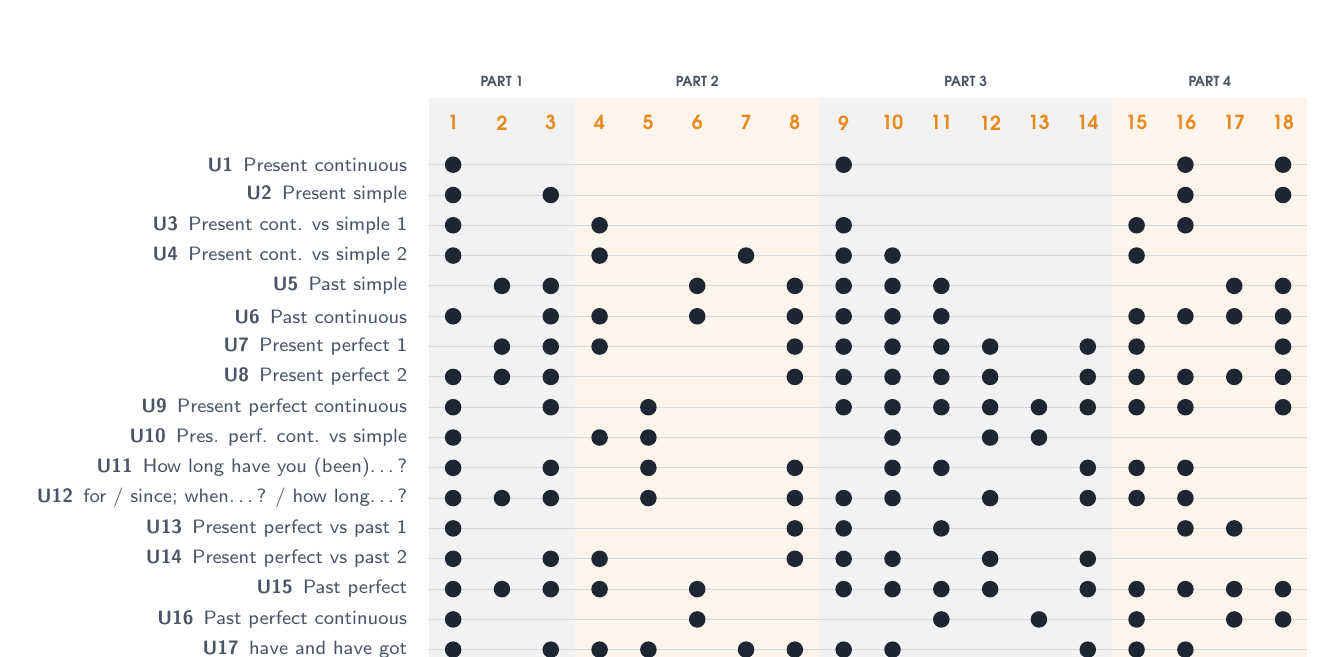
\begin{tikzpicture}[x=1mm,y=-1mm,font=\uifont\scriptsize]
\fill[ink!6] (40.00,-6.6) rectangle (58.60,65.85);
\node[font=\hfont\bfseries\tiny,text=inksoft] at (49.30,-8.7) {PART 1};
\fill[accent!9] (58.60,-6.6) rectangle (89.60,65.85);
\node[font=\hfont\bfseries\tiny,text=inksoft] at (74.10,-8.7) {PART 2};
\fill[ink!6] (89.60,-6.6) rectangle (126.80,65.85);
\node[font=\hfont\bfseries\tiny,text=inksoft] at (108.20,-8.7) {PART 3};
\fill[accent!9] (126.80,-6.6) rectangle (151.60,65.85);
\node[font=\hfont\bfseries\tiny,text=inksoft] at (139.20,-8.7) {PART 4};
\node[font=\hfont\bfseries\scriptsize,text=accent] at (43.10,-3.4) {1};
\node[font=\hfont\bfseries\scriptsize,text=accent] at (49.30,-3.4) {2};
\node[font=\hfont\bfseries\scriptsize,text=accent] at (55.50,-3.4) {3};
\node[font=\hfont\bfseries\scriptsize,text=accent] at (61.70,-3.4) {4};
\node[font=\hfont\bfseries\scriptsize,text=accent] at (67.90,-3.4) {5};
\node[font=\hfont\bfseries\scriptsize,text=accent] at (74.10,-3.4) {6};
\node[font=\hfont\bfseries\scriptsize,text=accent] at (80.30,-3.4) {7};
\node[font=\hfont\bfseries\scriptsize,text=accent] at (86.50,-3.4) {8};
\node[font=\hfont\bfseries\scriptsize,text=accent] at (92.70,-3.4) {9};
\node[font=\hfont\bfseries\scriptsize,text=accent] at (98.90,-3.4) {10};
\node[font=\hfont\bfseries\scriptsize,text=accent] at (105.10,-3.4) {11};
\node[font=\hfont\bfseries\scriptsize,text=accent] at (111.30,-3.4) {12};
\node[font=\hfont\bfseries\scriptsize,text=accent] at (117.50,-3.4) {13};
\node[font=\hfont\bfseries\scriptsize,text=accent] at (123.70,-3.4) {14};
\node[font=\hfont\bfseries\scriptsize,text=accent] at (129.90,-3.4) {15};
\node[font=\hfont\bfseries\scriptsize,text=accent] at (136.10,-3.4) {16};
\node[font=\hfont\bfseries\scriptsize,text=accent] at (142.30,-3.4) {17};
\node[font=\hfont\bfseries\scriptsize,text=accent] at (148.50,-3.4) {18};
\node[anchor=east,text=inksoft] at (38.50,1.93) {\textbf{U1}\enspace Present continuous};
\draw[line!70,line width=0.3pt] (40.00,1.93) -- (151.60,1.93);
\fill[ink] (43.10,1.93) circle (1.05);
\fill[ink] (92.70,1.93) circle (1.05);
\fill[ink] (136.10,1.93) circle (1.05);
\fill[ink] (148.50,1.93) circle (1.05);
\node[anchor=east,text=inksoft] at (38.50,5.78) {\textbf{U2}\enspace Present simple};
\draw[line!70,line width=0.3pt] (40.00,5.78) -- (151.60,5.78);
\fill[ink] (43.10,5.78) circle (1.05);
\fill[ink] (55.50,5.78) circle (1.05);
\fill[ink] (136.10,5.78) circle (1.05);
\fill[ink] (148.50,5.78) circle (1.05);
\node[anchor=east,text=inksoft] at (38.50,9.62) {\textbf{U3}\enspace Present cont. vs simple 1};
\draw[line!70,line width=0.3pt] (40.00,9.62) -- (151.60,9.62);
\fill[ink] (43.10,9.62) circle (1.05);
\fill[ink] (61.70,9.62) circle (1.05);
\fill[ink] (92.70,9.62) circle (1.05);
\fill[ink] (129.90,9.62) circle (1.05);
\fill[ink] (136.10,9.62) circle (1.05);
\node[anchor=east,text=inksoft] at (38.50,13.47) {\textbf{U4}\enspace Present cont. vs simple 2};
\draw[line!70,line width=0.3pt] (40.00,13.47) -- (151.60,13.47);
\fill[ink] (43.10,13.47) circle (1.05);
\fill[ink] (61.70,13.47) circle (1.05);
\fill[ink] (80.30,13.47) circle (1.05);
\fill[ink] (92.70,13.47) circle (1.05);
\fill[ink] (98.90,13.47) circle (1.05);
\fill[ink] (129.90,13.47) circle (1.05);
\node[anchor=east,text=inksoft] at (38.50,17.32) {\textbf{U5}\enspace Past simple};
\draw[line!70,line width=0.3pt] (40.00,17.32) -- (151.60,17.32);
\fill[ink] (49.30,17.32) circle (1.05);
\fill[ink] (55.50,17.32) circle (1.05);
\fill[ink] (74.10,17.32) circle (1.05);
\fill[ink] (86.50,17.32) circle (1.05);
\fill[ink] (92.70,17.32) circle (1.05);
\fill[ink] (98.90,17.32) circle (1.05);
\fill[ink] (105.10,17.32) circle (1.05);
\fill[ink] (142.30,17.32) circle (1.05);
\fill[ink] (148.50,17.32) circle (1.05);
\node[anchor=east,text=inksoft] at (38.50,21.18) {\textbf{U6}\enspace Past continuous};
\draw[line!70,line width=0.3pt] (40.00,21.18) -- (151.60,21.18);
\fill[ink] (43.10,21.18) circle (1.05);
\fill[ink] (55.50,21.18) circle (1.05);
\fill[ink] (61.70,21.18) circle (1.05);
\fill[ink] (74.10,21.18) circle (1.05);
\fill[ink] (86.50,21.18) circle (1.05);
\fill[ink] (92.70,21.18) circle (1.05);
\fill[ink] (98.90,21.18) circle (1.05);
\fill[ink] (105.10,21.18) circle (1.05);
\fill[ink] (129.90,21.18) circle (1.05);
\fill[ink] (136.10,21.18) circle (1.05);
\fill[ink] (142.30,21.18) circle (1.05);
\fill[ink] (148.50,21.18) circle (1.05);
\node[anchor=east,text=inksoft] at (38.50,25.03) {\textbf{U7}\enspace Present perfect 1};
\draw[line!70,line width=0.3pt] (40.00,25.03) -- (151.60,25.03);
\fill[ink] (49.30,25.03) circle (1.05);
\fill[ink] (55.50,25.03) circle (1.05);
\fill[ink] (61.70,25.03) circle (1.05);
\fill[ink] (86.50,25.03) circle (1.05);
\fill[ink] (92.70,25.03) circle (1.05);
\fill[ink] (98.90,25.03) circle (1.05);
\fill[ink] (105.10,25.03) circle (1.05);
\fill[ink] (111.30,25.03) circle (1.05);
\fill[ink] (123.70,25.03) circle (1.05);
\fill[ink] (129.90,25.03) circle (1.05);
\fill[ink] (148.50,25.03) circle (1.05);
\node[anchor=east,text=inksoft] at (38.50,28.88) {\textbf{U8}\enspace Present perfect 2};
\draw[line!70,line width=0.3pt] (40.00,28.88) -- (151.60,28.88);
\fill[ink] (43.10,28.88) circle (1.05);
\fill[ink] (49.30,28.88) circle (1.05);
\fill[ink] (55.50,28.88) circle (1.05);
\fill[ink] (86.50,28.88) circle (1.05);
\fill[ink] (92.70,28.88) circle (1.05);
\fill[ink] (98.90,28.88) circle (1.05);
\fill[ink] (105.10,28.88) circle (1.05);
\fill[ink] (111.30,28.88) circle (1.05);
\fill[ink] (123.70,28.88) circle (1.05);
\fill[ink] (129.90,28.88) circle (1.05);
\fill[ink] (136.10,28.88) circle (1.05);
\fill[ink] (142.30,28.88) circle (1.05);
\fill[ink] (148.50,28.88) circle (1.05);
\node[anchor=east,text=inksoft] at (38.50,32.73) {\textbf{U9}\enspace Present perfect continuous};
\draw[line!70,line width=0.3pt] (40.00,32.73) -- (151.60,32.73);
\fill[ink] (43.10,32.73) circle (1.05);
\fill[ink] (55.50,32.73) circle (1.05);
\fill[ink] (67.90,32.73) circle (1.05);
\fill[ink] (92.70,32.73) circle (1.05);
\fill[ink] (98.90,32.73) circle (1.05);
\fill[ink] (105.10,32.73) circle (1.05);
\fill[ink] (111.30,32.73) circle (1.05);
\fill[ink] (117.50,32.73) circle (1.05);
\fill[ink] (123.70,32.73) circle (1.05);
\fill[ink] (129.90,32.73) circle (1.05);
\fill[ink] (136.10,32.73) circle (1.05);
\fill[ink] (148.50,32.73) circle (1.05);
\node[anchor=east,text=inksoft] at (38.50,36.58) {\textbf{U10}\enspace Pres. perf. cont. vs simple};
\draw[line!70,line width=0.3pt] (40.00,36.58) -- (151.60,36.58);
\fill[ink] (43.10,36.58) circle (1.05);
\fill[ink] (61.70,36.58) circle (1.05);
\fill[ink] (67.90,36.58) circle (1.05);
\fill[ink] (98.90,36.58) circle (1.05);
\fill[ink] (111.30,36.58) circle (1.05);
\fill[ink] (117.50,36.58) circle (1.05);
\node[anchor=east,text=inksoft] at (38.50,40.43) {\textbf{U11}\enspace How long have you (been)…?};
\draw[line!70,line width=0.3pt] (40.00,40.43) -- (151.60,40.43);
\fill[ink] (43.10,40.43) circle (1.05);
\fill[ink] (55.50,40.43) circle (1.05);
\fill[ink] (67.90,40.43) circle (1.05);
\fill[ink] (86.50,40.43) circle (1.05);
\fill[ink] (98.90,40.43) circle (1.05);
\fill[ink] (105.10,40.43) circle (1.05);
\fill[ink] (123.70,40.43) circle (1.05);
\fill[ink] (129.90,40.43) circle (1.05);
\fill[ink] (136.10,40.43) circle (1.05);
\node[anchor=east,text=inksoft] at (38.50,44.27) {\textbf{U12}\enspace for / since; when…? / how long…?};
\draw[line!70,line width=0.3pt] (40.00,44.27) -- (151.60,44.27);
\fill[ink] (43.10,44.27) circle (1.05);
\fill[ink] (49.30,44.27) circle (1.05);
\fill[ink] (55.50,44.27) circle (1.05);
\fill[ink] (67.90,44.27) circle (1.05);
\fill[ink] (86.50,44.27) circle (1.05);
\fill[ink] (92.70,44.27) circle (1.05);
\fill[ink] (98.90,44.27) circle (1.05);
\fill[ink] (111.30,44.27) circle (1.05);
\fill[ink] (123.70,44.27) circle (1.05);
\fill[ink] (129.90,44.27) circle (1.05);
\fill[ink] (136.10,44.27) circle (1.05);
\node[anchor=east,text=inksoft] at (38.50,48.12) {\textbf{U13}\enspace Present perfect vs past 1};
\draw[line!70,line width=0.3pt] (40.00,48.12) -- (151.60,48.12);
\fill[ink] (43.10,48.12) circle (1.05);
\fill[ink] (86.50,48.12) circle (1.05);
\fill[ink] (92.70,48.12) circle (1.05);
\fill[ink] (105.10,48.12) circle (1.05);
\fill[ink] (136.10,48.12) circle (1.05);
\fill[ink] (142.30,48.12) circle (1.05);
\node[anchor=east,text=inksoft] at (38.50,51.98) {\textbf{U14}\enspace Present perfect vs past 2};
\draw[line!70,line width=0.3pt] (40.00,51.98) -- (151.60,51.98);
\fill[ink] (43.10,51.98) circle (1.05);
\fill[ink] (55.50,51.98) circle (1.05);
\fill[ink] (61.70,51.98) circle (1.05);
\fill[ink] (86.50,51.98) circle (1.05);
\fill[ink] (92.70,51.98) circle (1.05);
\fill[ink] (98.90,51.98) circle (1.05);
\fill[ink] (111.30,51.98) circle (1.05);
\fill[ink] (123.70,51.98) circle (1.05);
\node[anchor=east,text=inksoft] at (38.50,55.83) {\textbf{U15}\enspace Past perfect};
\draw[line!70,line width=0.3pt] (40.00,55.83) -- (151.60,55.83);
\fill[ink] (43.10,55.83) circle (1.05);
\fill[ink] (49.30,55.83) circle (1.05);
\fill[ink] (55.50,55.83) circle (1.05);
\fill[ink] (61.70,55.83) circle (1.05);
\fill[ink] (74.10,55.83) circle (1.05);
\fill[ink] (92.70,55.83) circle (1.05);
\fill[ink] (98.90,55.83) circle (1.05);
\fill[ink] (105.10,55.83) circle (1.05);
\fill[ink] (111.30,55.83) circle (1.05);
\fill[ink] (123.70,55.83) circle (1.05);
\fill[ink] (129.90,55.83) circle (1.05);
\fill[ink] (136.10,55.83) circle (1.05);
\fill[ink] (142.30,55.83) circle (1.05);
\fill[ink] (148.50,55.83) circle (1.05);
\node[anchor=east,text=inksoft] at (38.50,59.68) {\textbf{U16}\enspace Past perfect continuous};
\draw[line!70,line width=0.3pt] (40.00,59.68) -- (151.60,59.68);
\fill[ink] (43.10,59.68) circle (1.05);
\fill[ink] (74.10,59.68) circle (1.05);
\fill[ink] (105.10,59.68) circle (1.05);
\fill[ink] (117.50,59.68) circle (1.05);
\fill[ink] (129.90,59.68) circle (1.05);
\fill[ink] (142.30,59.68) circle (1.05);
\fill[ink] (148.50,59.68) circle (1.05);
\node[anchor=east,text=inksoft] at (38.50,63.52) {\textbf{U17}\enspace have and have got};
\draw[line!70,line width=0.3pt] (40.00,63.52) -- (151.60,63.52);
\fill[ink] (43.10,63.52) circle (1.05);
\fill[ink] (55.50,63.52) circle (1.05);
\fill[ink] (61.70,63.52) circle (1.05);
\fill[ink] (67.90,63.52) circle (1.05);
\fill[ink] (80.30,63.52) circle (1.05);
\fill[ink] (86.50,63.52) circle (1.05);
\fill[ink] (92.70,63.52) circle (1.05);
\fill[ink] (98.90,63.52) circle (1.05);
\fill[ink] (123.70,63.52) circle (1.05);
\fill[ink] (129.90,63.52) circle (1.05);
\fill[ink] (136.10,63.52) circle (1.05);
\end{tikzpicture}
\end{center}


\partbanner{1}{WARM-UP}{Quick retrieval. First instinct, then confidence.}

\exhead{1}{Snap decisions}{\upill{1}\,\upill{2}\,\upill{3}\,\upill{4}\,\upill{6}\,\upill{8}\,\upill{9}\,\upill{10}\,\upill{11}\,\upill{12}\,\upill{13}\,\upill{14}\,\upill{15}\,\upill{16}\,\upill{17}}{\cDailyI\,\cUniI\,\cLabI\,\cGameI\,\mTimed}
\instr{Choose the correct form. Go fast — about ten seconds per sentence. Then rate your confidence:
\tikz[baseline=-0.6ex]{\fill[mute] (0,0) circle (1.25mm);}~sure \quad
\tikz[baseline=-0.6ex]{\draw[mute,line width=0.5pt] (0,0) circle (1.25mm); \fill[mute] (0,1.25mm) arc (90:270:1.25mm) -- cycle;}~50/50 \quad
\tikz[baseline=-0.6ex]{\draw[mute,line width=0.5pt] (0,0) circle (1.25mm);}~guess. Circle one for each sentence.}
\vspace{2pt}
\noindent\begin{tabularx}{\linewidth}{@{}p{5mm}>{\RaggedRight\arraybackslash}X@{\hspace{4mm}}r@{}}\num{1} & Sorry, I can’t talk right now — I \opt{cook}{’m cooking} dinner. Can I call you back? & \conf\end{tabularx}\par\vspace{0.9mm}
\noindent\begin{tabularx}{\linewidth}{@{}p{5mm}>{\RaggedRight\arraybackslash}X@{\hspace{4mm}}r@{}}\num{2} & I \opt{’ve lost}{lost} my student card last week, but someone handed it in at reception. & \conf\end{tabularx}\par\vspace{0.9mm}
\noindent\begin{tabularx}{\linewidth}{@{}p{5mm}>{\RaggedRight\arraybackslash}X@{\hspace{4mm}}r@{}}\num{3} & \opt{Have you got}{Are you having} a spare HDMI cable? & \conf\end{tabularx}\par\vspace{0.9mm}
\noindent\begin{tabularx}{\linewidth}{@{}p{5mm}>{\RaggedRight\arraybackslash}X@{\hspace{4mm}}r@{}}\num{4} & When I looked outside, the sun was shining, but the streets were wet. It \opt{was raining}{had been raining}. & \conf\end{tabularx}\par\vspace{0.9mm}
\noindent\begin{tabularx}{\linewidth}{@{}p{5mm}>{\RaggedRight\arraybackslash}X@{\hspace{4mm}}r@{}}\num{5} & I \opt{always cycle}{’m always cycling} to campus — it’s faster than the bus. & \conf\end{tabularx}\par\vspace{0.9mm}
\noindent\begin{tabularx}{\linewidth}{@{}p{5mm}>{\RaggedRight\arraybackslash}X@{\hspace{4mm}}r@{}}\num{6} & How long \opt{are you}{have you been} in Belgium? & \conf\end{tabularx}\par\vspace{0.9mm}
\noindent\begin{tabularx}{\linewidth}{@{}p{5mm}>{\RaggedRight\arraybackslash}X@{\hspace{4mm}}r@{}}\num{7} & Who \opt{has invented}{invented} the transistor? & \conf\end{tabularx}\par\vspace{0.9mm}
\noindent\begin{tabularx}{\linewidth}{@{}p{5mm}>{\RaggedRight\arraybackslash}X@{\hspace{4mm}}r@{}}\num{8} & We \opt{’ve been sending}{’ve sent} over 300 messages in the group chat today, and nobody has started the report. & \conf\end{tabularx}\par\vspace{0.9mm}
\noindent\begin{tabularx}{\linewidth}{@{}p{5mm}>{\RaggedRight\arraybackslash}X@{\hspace{4mm}}r@{}}\num{9} & Tom \opt{is}{is being} really rude today. He’s normally so chill. & \conf\end{tabularx}\par\vspace{0.9mm}
\noindent\begin{tabularx}{\linewidth}{@{}p{5mm}>{\RaggedRight\arraybackslash}X@{\hspace{4mm}}r@{}}\num{10} & This is the first time I \opt{try}{’ve tried} waterzooi — it’s amazing! & \conf\end{tabularx}\par\vspace{0.9mm}
\noindent\begin{tabularx}{\linewidth}{@{}p{5mm}>{\RaggedRight\arraybackslash}X@{\hspace{4mm}}r@{}}\num{11} & I \opt{played}{was playing} ranked when my internet went down. & \conf\end{tabularx}\par\vspace{0.9mm}
\noindent\begin{tabularx}{\linewidth}{@{}p{5mm}>{\RaggedRight\arraybackslash}X@{\hspace{4mm}}r@{}}\num{12} & It’s been ages \opt{since}{for} we last played together. & \conf\end{tabularx}\par\vspace{0.9mm}
\noindent\begin{tabularx}{\linewidth}{@{}p{5mm}>{\RaggedRight\arraybackslash}X@{\hspace{4mm}}r@{}}\num{13} & Steel \opt{expands}{is expanding} when it gets hot, so bridges need expansion joints. & \conf\end{tabularx}\par\vspace{0.9mm}
\noindent\begin{tabularx}{\linewidth}{@{}p{5mm}>{\RaggedRight\arraybackslash}X@{\hspace{4mm}}r@{}}\num{14} & I didn’t recognise Ruben at first — he \opt{grew}{had grown} a beard. & \conf\end{tabularx}\par\vspace{0.9mm}
\noindent\begin{tabularx}{\linewidth}{@{}p{5mm}>{\RaggedRight\arraybackslash}X@{\hspace{4mm}}r@{}}\num{15} & Why are you out of breath? \opt{Have you run}{Have you been running}? & \conf\end{tabularx}\par\vspace{0.9mm}
\noindent\begin{tabularx}{\linewidth}{@{}p{5mm}>{\RaggedRight\arraybackslash}X@{\hspace{4mm}}r@{}}\num{16} & It’s 10:30. \opt{Did you see}{Have you seen} Marta this morning? & \conf\end{tabularx}\par\vspace{0.9mm}
\noindent\begin{tabularx}{\linewidth}{@{}p{5mm}>{\RaggedRight\arraybackslash}X@{\hspace{4mm}}r@{}}\num{17} & I \opt{’ve known}{’ve been knowing} Arne since our first week at uni. & \conf\end{tabularx}\par\vspace{0.9mm}
\noindent\begin{tabularx}{\linewidth}{@{}p{5mm}>{\RaggedRight\arraybackslash}X@{\hspace{4mm}}r@{}}\num{18} & We \opt{had}{had got} a dog when I was a kid. & \conf\end{tabularx}\par\vspace{0.9mm}
\noindent\begin{tabularx}{\linewidth}{@{}p{5mm}>{\RaggedRight\arraybackslash}X@{\hspace{4mm}}r@{}}\num{19} & Rents in Leuven \opt{rise}{are rising} so fast — mine went up again in September. & \conf\end{tabularx}\par\vspace{0.9mm}
\noindent\begin{tabularx}{\linewidth}{@{}p{5mm}>{\RaggedRight\arraybackslash}X@{\hspace{4mm}}r@{}}\num{20} & I \opt{’ve been writing}{’ve written} the intro of our report for three days, and it’s still not finished. & \conf\end{tabularx}\par\vspace{0.9mm}
\begin{speakbox}\textbf{Before you check:} read all twenty sentences aloud with your answers, at normal speaking speed. Any sentence that “sounds wrong” in your mouth? Put a small \textbf{?} next to it.\end{speakbox}


\exhead{2}{Crossword: forms on the fly}{\upill{5}\,\upill{7}\,\upill{8}\,\upill{12}\,\upill{15}}{\cDailyI\,\cUniI\,\cGameI\,\mThink}
\instr{Each clue is a sentence. Complete it with the \textbf{past simple} or the \textbf{past participle} of the verb in brackets, then write the word in the grid. Say the full sentence aloud as you go.}
\begin{center}
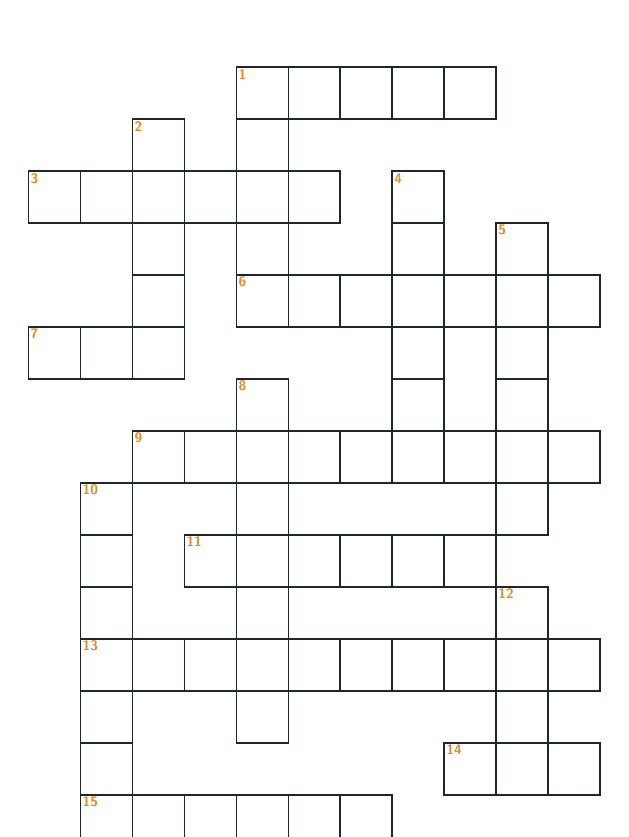
\begin{tikzpicture}[x=6.6mm,y=-6.6mm]
\fill[white] (1,11) rectangle +(1,1); \draw[ink,line width=0.6pt] (1,11) rectangle +(1,1);
\node[anchor=north west,inner sep=0.6pt,font=\uifont\bfseries\fontsize{5.5}{6}\selectfont,text=accent] at (1,11) {13};
\fill[white] (2,11) rectangle +(1,1); \draw[ink,line width=0.6pt] (2,11) rectangle +(1,1);
\fill[white] (3,11) rectangle +(1,1); \draw[ink,line width=0.6pt] (3,11) rectangle +(1,1);
\fill[white] (4,11) rectangle +(1,1); \draw[ink,line width=0.6pt] (4,11) rectangle +(1,1);
\fill[white] (5,11) rectangle +(1,1); \draw[ink,line width=0.6pt] (5,11) rectangle +(1,1);
\fill[white] (6,11) rectangle +(1,1); \draw[ink,line width=0.6pt] (6,11) rectangle +(1,1);
\fill[white] (7,11) rectangle +(1,1); \draw[ink,line width=0.6pt] (7,11) rectangle +(1,1);
\fill[white] (8,11) rectangle +(1,1); \draw[ink,line width=0.6pt] (8,11) rectangle +(1,1);
\fill[white] (9,11) rectangle +(1,1); \draw[ink,line width=0.6pt] (9,11) rectangle +(1,1);
\fill[white] (10,11) rectangle +(1,1); \draw[ink,line width=0.6pt] (10,11) rectangle +(1,1);
\fill[white] (4,6) rectangle +(1,1); \draw[ink,line width=0.6pt] (4,6) rectangle +(1,1);
\node[anchor=north west,inner sep=0.6pt,font=\uifont\bfseries\fontsize{5.5}{6}\selectfont,text=accent] at (4,6) {8};
\fill[white] (4,7) rectangle +(1,1); \draw[ink,line width=0.6pt] (4,7) rectangle +(1,1);
\fill[white] (4,8) rectangle +(1,1); \draw[ink,line width=0.6pt] (4,8) rectangle +(1,1);
\fill[white] (4,9) rectangle +(1,1); \draw[ink,line width=0.6pt] (4,9) rectangle +(1,1);
\fill[white] (4,10) rectangle +(1,1); \draw[ink,line width=0.6pt] (4,10) rectangle +(1,1);
\fill[white] (4,12) rectangle +(1,1); \draw[ink,line width=0.6pt] (4,12) rectangle +(1,1);
\fill[white] (2,7) rectangle +(1,1); \draw[ink,line width=0.6pt] (2,7) rectangle +(1,1);
\node[anchor=north west,inner sep=0.6pt,font=\uifont\bfseries\fontsize{5.5}{6}\selectfont,text=accent] at (2,7) {9};
\fill[white] (3,7) rectangle +(1,1); \draw[ink,line width=0.6pt] (3,7) rectangle +(1,1);
\fill[white] (5,7) rectangle +(1,1); \draw[ink,line width=0.6pt] (5,7) rectangle +(1,1);
\fill[white] (6,7) rectangle +(1,1); \draw[ink,line width=0.6pt] (6,7) rectangle +(1,1);
\fill[white] (7,7) rectangle +(1,1); \draw[ink,line width=0.6pt] (7,7) rectangle +(1,1);
\fill[white] (8,7) rectangle +(1,1); \draw[ink,line width=0.6pt] (8,7) rectangle +(1,1);
\fill[white] (9,7) rectangle +(1,1); \draw[ink,line width=0.6pt] (9,7) rectangle +(1,1);
\fill[white] (10,7) rectangle +(1,1); \draw[ink,line width=0.6pt] (10,7) rectangle +(1,1);
\fill[white] (1,8) rectangle +(1,1); \draw[ink,line width=0.6pt] (1,8) rectangle +(1,1);
\node[anchor=north west,inner sep=0.6pt,font=\uifont\bfseries\fontsize{5.5}{6}\selectfont,text=accent] at (1,8) {10};
\fill[white] (1,9) rectangle +(1,1); \draw[ink,line width=0.6pt] (1,9) rectangle +(1,1);
\fill[white] (1,10) rectangle +(1,1); \draw[ink,line width=0.6pt] (1,10) rectangle +(1,1);
\fill[white] (1,12) rectangle +(1,1); \draw[ink,line width=0.6pt] (1,12) rectangle +(1,1);
\fill[white] (1,13) rectangle +(1,1); \draw[ink,line width=0.6pt] (1,13) rectangle +(1,1);
\fill[white] (1,14) rectangle +(1,1); \draw[ink,line width=0.6pt] (1,14) rectangle +(1,1);
\node[anchor=north west,inner sep=0.6pt,font=\uifont\bfseries\fontsize{5.5}{6}\selectfont,text=accent] at (1,14) {15};
\fill[white] (3,9) rectangle +(1,1); \draw[ink,line width=0.6pt] (3,9) rectangle +(1,1);
\node[anchor=north west,inner sep=0.6pt,font=\uifont\bfseries\fontsize{5.5}{6}\selectfont,text=accent] at (3,9) {11};
\fill[white] (5,9) rectangle +(1,1); \draw[ink,line width=0.6pt] (5,9) rectangle +(1,1);
\fill[white] (6,9) rectangle +(1,1); \draw[ink,line width=0.6pt] (6,9) rectangle +(1,1);
\fill[white] (7,9) rectangle +(1,1); \draw[ink,line width=0.6pt] (7,9) rectangle +(1,1);
\fill[white] (8,9) rectangle +(1,1); \draw[ink,line width=0.6pt] (8,9) rectangle +(1,1);
\fill[white] (2,14) rectangle +(1,1); \draw[ink,line width=0.6pt] (2,14) rectangle +(1,1);
\fill[white] (3,14) rectangle +(1,1); \draw[ink,line width=0.6pt] (3,14) rectangle +(1,1);
\fill[white] (4,14) rectangle +(1,1); \draw[ink,line width=0.6pt] (4,14) rectangle +(1,1);
\fill[white] (5,14) rectangle +(1,1); \draw[ink,line width=0.6pt] (5,14) rectangle +(1,1);
\fill[white] (6,14) rectangle +(1,1); \draw[ink,line width=0.6pt] (6,14) rectangle +(1,1);
\fill[white] (9,3) rectangle +(1,1); \draw[ink,line width=0.6pt] (9,3) rectangle +(1,1);
\node[anchor=north west,inner sep=0.6pt,font=\uifont\bfseries\fontsize{5.5}{6}\selectfont,text=accent] at (9,3) {5};
\fill[white] (9,4) rectangle +(1,1); \draw[ink,line width=0.6pt] (9,4) rectangle +(1,1);
\fill[white] (9,5) rectangle +(1,1); \draw[ink,line width=0.6pt] (9,5) rectangle +(1,1);
\fill[white] (9,6) rectangle +(1,1); \draw[ink,line width=0.6pt] (9,6) rectangle +(1,1);
\fill[white] (9,8) rectangle +(1,1); \draw[ink,line width=0.6pt] (9,8) rectangle +(1,1);
\fill[white] (4,4) rectangle +(1,1); \draw[ink,line width=0.6pt] (4,4) rectangle +(1,1);
\node[anchor=north west,inner sep=0.6pt,font=\uifont\bfseries\fontsize{5.5}{6}\selectfont,text=accent] at (4,4) {6};
\fill[white] (5,4) rectangle +(1,1); \draw[ink,line width=0.6pt] (5,4) rectangle +(1,1);
\fill[white] (6,4) rectangle +(1,1); \draw[ink,line width=0.6pt] (6,4) rectangle +(1,1);
\fill[white] (7,4) rectangle +(1,1); \draw[ink,line width=0.6pt] (7,4) rectangle +(1,1);
\fill[white] (8,4) rectangle +(1,1); \draw[ink,line width=0.6pt] (8,4) rectangle +(1,1);
\fill[white] (10,4) rectangle +(1,1); \draw[ink,line width=0.6pt] (10,4) rectangle +(1,1);
\fill[white] (7,2) rectangle +(1,1); \draw[ink,line width=0.6pt] (7,2) rectangle +(1,1);
\node[anchor=north west,inner sep=0.6pt,font=\uifont\bfseries\fontsize{5.5}{6}\selectfont,text=accent] at (7,2) {4};
\fill[white] (7,3) rectangle +(1,1); \draw[ink,line width=0.6pt] (7,3) rectangle +(1,1);
\fill[white] (7,5) rectangle +(1,1); \draw[ink,line width=0.6pt] (7,5) rectangle +(1,1);
\fill[white] (7,6) rectangle +(1,1); \draw[ink,line width=0.6pt] (7,6) rectangle +(1,1);
\fill[white] (4,0) rectangle +(1,1); \draw[ink,line width=0.6pt] (4,0) rectangle +(1,1);
\node[anchor=north west,inner sep=0.6pt,font=\uifont\bfseries\fontsize{5.5}{6}\selectfont,text=accent] at (4,0) {1};
\fill[white] (4,1) rectangle +(1,1); \draw[ink,line width=0.6pt] (4,1) rectangle +(1,1);
\fill[white] (4,2) rectangle +(1,1); \draw[ink,line width=0.6pt] (4,2) rectangle +(1,1);
\fill[white] (4,3) rectangle +(1,1); \draw[ink,line width=0.6pt] (4,3) rectangle +(1,1);
\fill[white] (0,2) rectangle +(1,1); \draw[ink,line width=0.6pt] (0,2) rectangle +(1,1);
\node[anchor=north west,inner sep=0.6pt,font=\uifont\bfseries\fontsize{5.5}{6}\selectfont,text=accent] at (0,2) {3};
\fill[white] (1,2) rectangle +(1,1); \draw[ink,line width=0.6pt] (1,2) rectangle +(1,1);
\fill[white] (2,2) rectangle +(1,1); \draw[ink,line width=0.6pt] (2,2) rectangle +(1,1);
\fill[white] (3,2) rectangle +(1,1); \draw[ink,line width=0.6pt] (3,2) rectangle +(1,1);
\fill[white] (5,2) rectangle +(1,1); \draw[ink,line width=0.6pt] (5,2) rectangle +(1,1);
\fill[white] (5,0) rectangle +(1,1); \draw[ink,line width=0.6pt] (5,0) rectangle +(1,1);
\fill[white] (6,0) rectangle +(1,1); \draw[ink,line width=0.6pt] (6,0) rectangle +(1,1);
\fill[white] (7,0) rectangle +(1,1); \draw[ink,line width=0.6pt] (7,0) rectangle +(1,1);
\fill[white] (8,0) rectangle +(1,1); \draw[ink,line width=0.6pt] (8,0) rectangle +(1,1);
\fill[white] (2,1) rectangle +(1,1); \draw[ink,line width=0.6pt] (2,1) rectangle +(1,1);
\node[anchor=north west,inner sep=0.6pt,font=\uifont\bfseries\fontsize{5.5}{6}\selectfont,text=accent] at (2,1) {2};
\fill[white] (2,3) rectangle +(1,1); \draw[ink,line width=0.6pt] (2,3) rectangle +(1,1);
\fill[white] (2,4) rectangle +(1,1); \draw[ink,line width=0.6pt] (2,4) rectangle +(1,1);
\fill[white] (2,5) rectangle +(1,1); \draw[ink,line width=0.6pt] (2,5) rectangle +(1,1);
\fill[white] (9,10) rectangle +(1,1); \draw[ink,line width=0.6pt] (9,10) rectangle +(1,1);
\node[anchor=north west,inner sep=0.6pt,font=\uifont\bfseries\fontsize{5.5}{6}\selectfont,text=accent] at (9,10) {12};
\fill[white] (9,12) rectangle +(1,1); \draw[ink,line width=0.6pt] (9,12) rectangle +(1,1);
\fill[white] (9,13) rectangle +(1,1); \draw[ink,line width=0.6pt] (9,13) rectangle +(1,1);
\fill[white] (0,5) rectangle +(1,1); \draw[ink,line width=0.6pt] (0,5) rectangle +(1,1);
\node[anchor=north west,inner sep=0.6pt,font=\uifont\bfseries\fontsize{5.5}{6}\selectfont,text=accent] at (0,5) {7};
\fill[white] (1,5) rectangle +(1,1); \draw[ink,line width=0.6pt] (1,5) rectangle +(1,1);
\fill[white] (8,13) rectangle +(1,1); \draw[ink,line width=0.6pt] (8,13) rectangle +(1,1);
\node[anchor=north west,inner sep=0.6pt,font=\uifont\bfseries\fontsize{5.5}{6}\selectfont,text=accent] at (8,13) {14};
\fill[white] (10,13) rectangle +(1,1); \draw[ink,line width=0.6pt] (10,13) rectangle +(1,1);
\end{tikzpicture}
\end{center}
\vspace{-2mm}
\begin{multicols}{2}
{\hfont\bfseries\small\color{accent} ACROSS}
\begin{itemize}[leftmargin=7mm,itemsep=2.2pt,labelsep=2mm]\small
\item[\num{1}] Last night we \blank{} (spend) three hours looking for one missing semicolon.
\item[\num{3}] My game has \blank{} (freeze) — I can’t move!
\item[\num{6}] I \blank{} (think) the exam was at ten, but it had started at nine!
\item[\num{7}] We’ve \blank{} (win) five games in a row — don’t jinx it!
\item[\num{9}] I’ve \blank{} (forget) my password for the third time this week.
\item[\num{11}] Someone has \blank{} (steal) my bike saddle. Welcome to Leuven!
\item[\num{13}] I had never really \blank{} (understand) Fourier series until the TA drew them.
\item[\num{14}] We \blank{} (meet) in the first-year chemistry lab.
\item[\num{15}] Who \blank{} (teach) you to play Lúcio like that?
\end{itemize}
\columnbreak
{\hfont\bfseries\small\color{accent} DOWN}
\begin{itemize}[leftmargin=7mm,itemsep=2.2pt,labelsep=2mm]\small
\item[\num{1}] I haven’t \blank{} (sleep) properly since the exam period started.
\item[\num{2}] I’ve only just \blank{} (wake) up — give me five minutes.
\item[\num{4}] “Sorry, you’ve \blank{} (catch) me at a bad time. Can I call you back?”
\item[\num{5}] Have you \blank{} (choose) your electives for next semester yet?
\item[\num{8}] I’ve \blank{} (write) three lab reports this week — my wrist hurts.
\item[\num{10}] Has anyone \blank{} (bring) snacks for the study session?
\item[\num{12}] “Where’s Jonas?” “He’s \blank{} (go) to the shop. He’ll be back in ten.”
\end{itemize}
\end{multicols}


\exhead{3}{Questions in the wild}{\upill{2}\,\upill{5}\,\upill{6}\,\upill{7}\,\upill{8}\,\upill{9}\,\upill{11}\,\upill{12}\,\upill{14}\,\upill{15}\,\upill{17}}{\cDailyI\,\cUniI\,\mWrite\,\mSpeak}
\instr{Put the words in order to make questions you could hear in your first weeks back. Then answer each one \textbf{out loud}, truthfully, in one breath (start within three seconds).}
\begin{multicols}{2}
\num{1}\enspace {\uifont\small back\,\textcolor{mute}{/}\, Leuven\,\textcolor{mute}{/}\, long\,\textcolor{mute}{/}\, in\,\textcolor{mute}{/}\, you\,\textcolor{mute}{/}\, have\,\textcolor{mute}{/}\, been\,\textcolor{mute}{/}\, how}\par\vspace{0.3mm}\hspace*{5mm}\wfill\par\vspace{2.2mm}
\num{2}\enspace {\uifont\small Ardennes\,\textcolor{mute}{/}\, been\,\textcolor{mute}{/}\, ever\,\textcolor{mute}{/}\, the\,\textcolor{mute}{/}\, to\,\textcolor{mute}{/}\, you\,\textcolor{mute}{/}\, have}\par\vspace{0.3mm}\hspace*{5mm}\wfill\par\vspace{2.2mm}
\num{3}\enspace {\uifont\small summer\,\textcolor{mute}{/}\, up\,\textcolor{mute}{/}\, to\,\textcolor{mute}{/}\, since\,\textcolor{mute}{/}\, been\,\textcolor{mute}{/}\, you\,\textcolor{mute}{/}\, the\,\textcolor{mute}{/}\, what\,\textcolor{mute}{/}\, have}\par\vspace{0.3mm}\hspace*{5mm}\wfill\par\vspace{2.2mm}
\num{4}\enspace {\uifont\small gym\,\textcolor{mute}{/}\, you\,\textcolor{mute}{/}\, how\,\textcolor{mute}{/}\, go\,\textcolor{mute}{/}\, do\,\textcolor{mute}{/}\, to\,\textcolor{mute}{/}\, the\,\textcolor{mute}{/}\, often}\par\vspace{0.3mm}\hspace*{5mm}\wfill\par\vspace{2.2mm}
\num{5}\enspace {\uifont\small happened\,\textcolor{mute}{/}\, were\,\textcolor{mute}{/}\, doing\,\textcolor{mute}{/}\, blackout\,\textcolor{mute}{/}\, you\,\textcolor{mute}{/}\, the\,\textcolor{mute}{/}\, when\,\textcolor{mute}{/}\, what}\par\vspace{0.3mm}\hspace*{5mm}\wfill\par\vspace{2.2mm}
\num{6}\enspace {\uifont\small timetable\,\textcolor{mute}{/}\, checked\,\textcolor{mute}{/}\, yet\,\textcolor{mute}{/}\, the\,\textcolor{mute}{/}\, exam\,\textcolor{mute}{/}\, have\,\textcolor{mute}{/}\, you}\par\vspace{0.3mm}\hspace*{5mm}\wfill\par\vspace{2.2mm}
\num{7}\enspace {\uifont\small bed\,\textcolor{mute}{/}\, last\,\textcolor{mute}{/}\, go\,\textcolor{mute}{/}\, you\,\textcolor{mute}{/}\, time\,\textcolor{mute}{/}\, to\,\textcolor{mute}{/}\, did\,\textcolor{mute}{/}\, what\,\textcolor{mute}{/}\, night}\par\vspace{0.3mm}\hspace*{5mm}\wfill\par\vspace{2.2mm}
\num{8}\enspace {\uifont\small spare\,\textcolor{mute}{/}\, you\,\textcolor{mute}{/}\, a\,\textcolor{mute}{/}\, pen\,\textcolor{mute}{/}\, have\,\textcolor{mute}{/}\, got}\par\vspace{0.3mm}\hspace*{5mm}\wfill\par\vspace{2.2mm}
\num{9}\enspace {\uifont\small arrived\,\textcolor{mute}{/}\, started\,\textcolor{mute}{/}\, lecture\,\textcolor{mute}{/}\, you\,\textcolor{mute}{/}\, had\,\textcolor{mute}{/}\, already\,\textcolor{mute}{/}\, when\,\textcolor{mute}{/}\, the}\par\vspace{0.3mm}\hspace*{5mm}\wfill\par\vspace{2.2mm}
\num{10}\enspace {\uifont\small Dutch\,\textcolor{mute}{/}\, learning\,\textcolor{mute}{/}\, you\,\textcolor{mute}{/}\, long\,\textcolor{mute}{/}\, been\,\textcolor{mute}{/}\, have\,\textcolor{mute}{/}\, how}\par\vspace{0.3mm}\hspace*{5mm}\wfill\par\vspace{2.2mm}
\end{multicols}


\partbanner{2}{AIM TRAINING}{Precision shots: often both forms are grammatical — the meaning decides.}

\exhead{4}{Same words, different story}{\upill{3}\,\upill{4}\,\upill{6}\,\upill{7}\,\upill{10}\,\upill{14}\,\upill{15}\,\upill{17}}{\cDailyI\,\cUniI\,\cLabI\,\cGameI\,\mThink}
\instr{Each pair is almost identical — but the grammar changes the story. Draw lines to connect each sentence (\textbf{a}/\textbf{b}) with the continuation or situation (\textbf{i}/\textbf{ii}) that fits it.}
\vspace{1mm}
\needsp{3\baselineskip}\noindent\begin{tabularx}{\linewidth}{@{}p{5mm}X@{\hspace{2mm}}c@{\hspace{9mm}}c@{\hspace{2mm}}X@{}}
\num{1} & \textbf{a}\enspace I’ve lived in Leuven for two years. & \dotL & \dotL & \textbf{i}\enspace And honestly, I still love it here. \\[1.5pt]
 & \textbf{b}\enspace I lived in Leuven for two years. & \dotL & \dotL & \textbf{ii}\enspace Then I moved to Antwerp for my internship.
\end{tabularx}\par\vspace{1.2mm}{\color{line!60}\hrule height 0.3pt}\vspace{1.4mm}
\needsp{3\baselineskip}\noindent\begin{tabularx}{\linewidth}{@{}p{5mm}X@{\hspace{2mm}}c@{\hspace{9mm}}c@{\hspace{2mm}}X@{}}
\num{2} & \textbf{a}\enspace When I got to the lab, the TA was leaving. & \dotL & \dotL & \textbf{i}\enspace So I didn’t see her at all. \\[1.5pt]
 & \textbf{b}\enspace When I got to the lab, the TA had left. & \dotL & \dotL & \textbf{ii}\enspace So I managed to ask her one quick question at the door.
\end{tabularx}\par\vspace{1.2mm}{\color{line!60}\hrule height 0.3pt}\vspace{1.4mm}
\needsp{3\baselineskip}\noindent\begin{tabularx}{\linewidth}{@{}p{5mm}X@{\hspace{2mm}}c@{\hspace{9mm}}c@{\hspace{2mm}}X@{}}
\num{3} & \textbf{a}\enspace I’ve been fixing the 3D printer. & \dotL & \dotL & \textbf{i}\enspace That’s why my hands are covered in grease. It still doesn’t work, though. \\[1.5pt]
 & \textbf{b}\enspace I’ve fixed the 3D printer. & \dotL & \dotL & \textbf{ii}\enspace It works now — go and print your part.
\end{tabularx}\par\vspace{1.2mm}{\color{line!60}\hrule height 0.3pt}\vspace{1.4mm}
\needsp{3\baselineskip}\noindent\begin{tabularx}{\linewidth}{@{}p{5mm}X@{\hspace{2mm}}c@{\hspace{9mm}}c@{\hspace{2mm}}X@{}}
\num{4} & \textbf{a}\enspace Mila always borrows my calculator before exams. & \dotL & \dotL & \textbf{i}\enspace Honestly, she should just buy her own. \\[1.5pt]
 & \textbf{b}\enspace Mila is always borrowing my calculator. & \dotL & \dotL & \textbf{ii}\enspace It’s become a kind of good-luck ritual, and I don’t mind.
\end{tabularx}\par\vspace{1.2mm}{\color{line!60}\hrule height 0.3pt}\vspace{1.4mm}
\needsp{3\baselineskip}\noindent\begin{tabularx}{\linewidth}{@{}p{5mm}X@{\hspace{2mm}}c@{\hspace{9mm}}c@{\hspace{2mm}}X@{}}
\num{5} & \textbf{a}\enspace What do you think of the new hero? & \dotL & \dotL & \textbf{i}\enspace You look miles away. \\[1.5pt]
 & \textbf{b}\enspace What are you thinking about? & \dotL & \dotL & \textbf{ii}\enspace Is she worth learning for ranked?
\end{tabularx}\par\vspace{1.2mm}{\color{line!60}\hrule height 0.3pt}\vspace{1.4mm}
\needsp{3\baselineskip}\noindent\begin{tabularx}{\linewidth}{@{}p{5mm}X@{\hspace{2mm}}c@{\hspace{9mm}}c@{\hspace{2mm}}X@{}}
\num{6} & \textbf{a}\enspace Tom is selfish. & \dotL & \dotL & \textbf{i}\enspace He never shares anything with anyone. \\[1.5pt]
 & \textbf{b}\enspace Tom is being selfish. & \dotL & \dotL & \textbf{ii}\enspace He isn’t usually like this — he must be stressed about the exam.
\end{tabularx}\par\vspace{1.2mm}{\color{line!60}\hrule height 0.3pt}\vspace{1.4mm}
\needsp{3\baselineskip}\noindent\begin{tabularx}{\linewidth}{@{}p{5mm}X@{\hspace{2mm}}c@{\hspace{9mm}}c@{\hspace{2mm}}X@{}}
\num{7} & \textbf{a}\enspace When Leo called, I had dinner. & \dotL & \dotL & \textbf{i}\enspace I was in the middle of eating, so I didn’t pick up. \\[1.5pt]
 & \textbf{b}\enspace When Leo called, I was having dinner. & \dotL & \dotL & \textbf{ii}\enspace We talked for a bit, and then I ate.
\end{tabularx}\par\vspace{1.2mm}{\color{line!60}\hrule height 0.3pt}\vspace{1.4mm}
\needsp{3\baselineskip}\noindent\begin{tabularx}{\linewidth}{@{}p{5mm}X@{\hspace{2mm}}c@{\hspace{9mm}}c@{\hspace{2mm}}X@{}}
\num{8} & \textbf{a}\enspace Jonas has gone to Brazil. & \dotL & \dotL & \textbf{i}\enspace He’ll be back in September. \\[1.5pt]
 & \textbf{b}\enspace Jonas has been to Brazil. & \dotL & \dotL & \textbf{ii}\enspace He showed me his photos of Rio yesterday.
\end{tabularx}\par\vspace{1.2mm}{\color{line!60}\hrule height 0.3pt}\vspace{1.4mm}
\needsp{3\baselineskip}\noindent\begin{tabularx}{\linewidth}{@{}p{5mm}X@{\hspace{2mm}}c@{\hspace{9mm}}c@{\hspace{2mm}}X@{}}
\num{9} & \textbf{a}\enspace When the match ended, I logged off. & \dotL & \dotL & \textbf{i}\enspace I missed the final fight — I’d rage-quit after the second round. \\[1.5pt]
 & \textbf{b}\enspace When the match ended, I had logged off. & \dotL & \dotL & \textbf{ii}\enspace I stayed till the end, then went to bed.
\end{tabularx}\par\vspace{1.2mm}{\color{line!60}\hrule height 0.3pt}\vspace{1.4mm}
\needsp{3\baselineskip}\noindent\begin{tabularx}{\linewidth}{@{}p{5mm}X@{\hspace{2mm}}c@{\hspace{9mm}}c@{\hspace{2mm}}X@{}}
\num{10} & \textbf{a}\enspace They’re having a barbecue. & \dotL & \dotL & \textbf{i}\enspace Want to join? I can smell it from here. \\[1.5pt]
 & \textbf{b}\enspace They have a barbecue. & \dotL & \dotL & \textbf{ii}\enspace It’s in the garden, but they never use it.
\end{tabularx}\par\vspace{1.2mm}{\color{line!60}\hrule height 0.3pt}\vspace{1.4mm}
\needsp{3\baselineskip}\noindent\begin{tabularx}{\linewidth}{@{}p{5mm}X@{\hspace{2mm}}c@{\hspace{9mm}}c@{\hspace{2mm}}X@{}}
\num{11} & \textbf{a}\enspace I haven’t seen Marta this morning. & \dotL & \dotL & \textbf{i}\enspace Said at 4 p.m. \\[1.5pt]
 & \textbf{b}\enspace I didn’t see Marta this morning. & \dotL & \dotL & \textbf{ii}\enspace Said at 10 a.m.
\end{tabularx}\par\vspace{1.2mm}{\color{line!60}\hrule height 0.3pt}\vspace{1.4mm}

\exhead{5}{One situation, two angles}{\upill{9}\,\upill{10}\,\upill{11}\,\upill{12}\,\upill{17}}{\cDailyI\,\cUniI\,\cLabI\,\cGameI\,\mWrite}
\instr{For each situation write two sentences: the first about the \textbf{activity and how long} (present perfect continuous, where possible), the second about the \textbf{result} — how much or how many (present perfect simple). Careful: in two situations the verb doesn’t like continuous forms.}
\vspace{1mm}
\needsp{4\baselineskip}\noindent\num{1}\enspace{\uifont\small you \mdot{} revise for the thermodynamics exam \mdot{} since 9 a.m. \enspace\textcolor{accent}{$\vert$}\enspace cover \mdot{} four chapters}\par
\vspace{0.5mm}\noindent\hspace*{5mm}\textcolor{mute}{\scriptsize\uifont HOW LONG}\enspace\wfill\par\vspace{2.4mm}
\noindent\hspace*{5mm}\textcolor{mute}{\scriptsize\uifont RESULT}\hspace{4.1mm}\wfill\par\vspace{2.6mm}
\needsp{4\baselineskip}\noindent\num{2}\enspace{\uifont\small Wout \mdot{} play ranked \mdot{} all evening \enspace\textcolor{accent}{$\vert$}\enspace lose \mdot{} six games in a row}\par
\vspace{0.5mm}\noindent\hspace*{5mm}\textcolor{mute}{\scriptsize\uifont HOW LONG}\enspace\wfill\par\vspace{2.4mm}
\noindent\hspace*{5mm}\textcolor{mute}{\scriptsize\uifont RESULT}\hspace{4.1mm}\wfill\par\vspace{2.6mm}
\needsp{4\baselineskip}\noindent\num{3}\enspace{\uifont\small we \mdot{} try to fix this bug \mdot{} for two hours \enspace\textcolor{accent}{$\vert$}\enspace find \mdot{} three new bugs}\par
\vspace{0.5mm}\noindent\hspace*{5mm}\textcolor{mute}{\scriptsize\uifont HOW LONG}\enspace\wfill\par\vspace{2.4mm}
\noindent\hspace*{5mm}\textcolor{mute}{\scriptsize\uifont RESULT}\hspace{4.1mm}\wfill\par\vspace{2.6mm}
\needsp{4\baselineskip}\noindent\num{4}\enspace{\uifont\small my housemate \mdot{} cook \mdot{} since lunchtime \enspace\textcolor{accent}{$\vert$}\enspace make \mdot{} enough lasagne for ten people}\par
\vspace{0.5mm}\noindent\hspace*{5mm}\textcolor{mute}{\scriptsize\uifont HOW LONG}\enspace\wfill\par\vspace{2.4mm}
\noindent\hspace*{5mm}\textcolor{mute}{\scriptsize\uifont RESULT}\hspace{4.1mm}\wfill\par\vspace{2.6mm}
\needsp{4\baselineskip}\noindent\num{5}\enspace{\uifont\small I \mdot{} have this laptop \mdot{} since 2021 \enspace\textcolor{accent}{$\vert$}\enspace it \mdot{} crash \mdot{} three times this week}\par
\vspace{0.5mm}\noindent\hspace*{5mm}\textcolor{mute}{\scriptsize\uifont HOW LONG}\enspace\wfill\par\vspace{2.4mm}
\noindent\hspace*{5mm}\textcolor{mute}{\scriptsize\uifont RESULT}\hspace{4.1mm}\wfill\par\vspace{2.6mm}
\needsp{4\baselineskip}\noindent\num{6}\enspace{\uifont\small I \mdot{} learn Dutch \mdot{} for two years \enspace\textcolor{accent}{$\vert$}\enspace learn \mdot{} about 2,000 words}\par
\vspace{0.5mm}\noindent\hspace*{5mm}\textcolor{mute}{\scriptsize\uifont HOW LONG}\enspace\wfill\par\vspace{2.4mm}
\noindent\hspace*{5mm}\textcolor{mute}{\scriptsize\uifont RESULT}\hspace{4.1mm}\wfill\par\vspace{2.6mm}
\needsp{4\baselineskip}\noindent\num{7}\enspace{\uifont\small Ines and I \mdot{} know each other \mdot{} since primary school \enspace\textcolor{accent}{$\vert$}\enspace she \mdot{} visit me in Leuven \mdot{} twice}\par
\vspace{0.5mm}\noindent\hspace*{5mm}\textcolor{mute}{\scriptsize\uifont HOW LONG}\enspace\wfill\par\vspace{2.4mm}
\noindent\hspace*{5mm}\textcolor{mute}{\scriptsize\uifont RESULT}\hspace{4.1mm}\wfill\par\vspace{2.6mm}
\needsp{4\baselineskip}\noindent\num{8}\enspace{\uifont\small I \mdot{} train for a half-marathon \mdot{} since September \enspace\textcolor{accent}{$\vert$}\enspace run \mdot{} over 300 km}\par
\vspace{0.5mm}\noindent\hspace*{5mm}\textcolor{mute}{\scriptsize\uifont HOW LONG}\enspace\wfill\par\vspace{2.4mm}
\noindent\hspace*{5mm}\textcolor{mute}{\scriptsize\uifont RESULT}\hspace{4.1mm}\wfill\par\vspace{2.6mm}

\exhead{6}{The Monday from hell}{\upill{5}\,\upill{6}\,\upill{15}\,\upill{16}}{\cUniI\,\cLabI\,\cGameI\,\mWrite}
\instr{Look at Tiago’s Monday. Answer the questions in full sentences. Each answer needs a different past form — think about \emph{which moment} you are looking from.}

\begin{center}
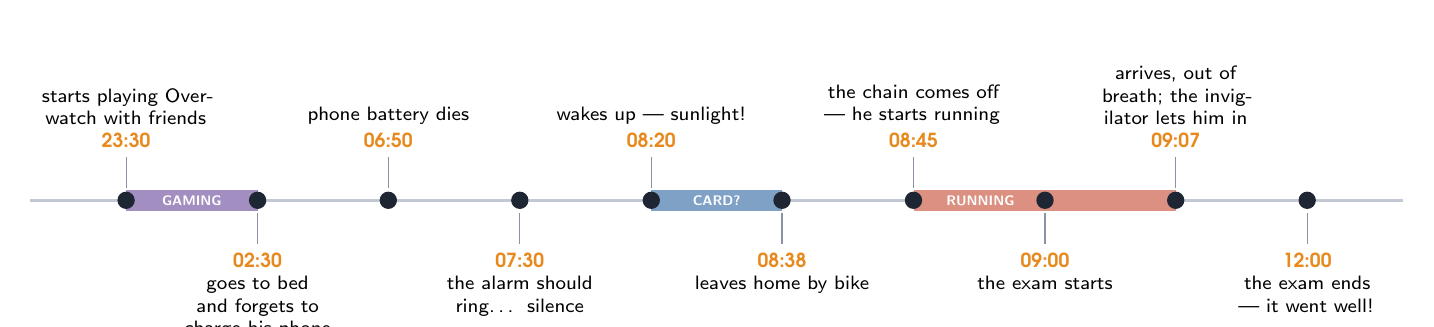
\begin{tikzpicture}[x=1mm,y=1mm,font=\uifont\scriptsize]
  % axis
  \draw[line,line width=1.2pt] (0.8,0) -- (175.2,0);
  % activity bars
  \fill[cGame!70] (13,-1.3) rectangle (29.7,1.3);
  \fill[cUni!65] (79.7,-1.3) rectangle (96.3,1.3);
  \fill[cLab!65] (113,-1.3) rectangle (146.3,1.3);
  % markers above the axis
  \foreach \x/\t/\txt in {
     13/23:30/{starts playing Overwatch with friends},
     46.3/06:50/{phone battery dies},
     79.7/08:20/{wakes up — sunlight!},
     113/08:45/{the chain comes off — he starts running},
     146.3/09:07/{arrives, out of breath; the invigilator lets him in}}
  {
     \fill[ink] (\x,0) circle (1.1);
     \draw[mute,line width=0.4pt] (\x,1.6) -- (\x,5.5);
     \node[font=\hfont\bfseries\scriptsize,text=accent] at (\x,7.6) {\t};
     \node[text width=25mm,align=center,anchor=south,inner sep=0pt] at (\x,9.6) {\txt};
  }
  % markers below the axis
  \foreach \x/\t/\txt in {
     29.7/02:30/{goes to bed and forgets to charge his phone},
     63/07:30/{the alarm should ring\dots{} silence},
     96.3/08:38/{leaves home by bike},
     129.7/09:00/{the exam starts},
     163/12:00/{the exam ends — it went well!}}
  {
     \fill[ink] (\x,0) circle (1.1);
     \draw[mute,line width=0.4pt] (\x,-1.6) -- (\x,-5.5);
     \node[font=\hfont\bfseries\scriptsize,text=accent] at (\x,-7.6) {\t};
     \node[text width=25mm,align=center,anchor=north,inner sep=0pt] at (\x,-9.6) {\txt};
  }
  \node[font=\uifont\tiny\bfseries,text=white] at (21.35,0) {GAMING};
  \node[font=\uifont\tiny\bfseries,text=white] at (88,0) {CARD?};
  \node[font=\uifont\tiny\bfseries,text=white] at (121.5,0) {RUNNING};
\end{tikzpicture}
\end{center}
\num{1}\enspace Why didn’t Tiago’s alarm go off?\par\vspace{0.4mm}\noindent\hspace*{5mm}\wfill\par\vspace{2.6mm}
\num{2}\enspace What had he been doing until 2:30 a.m.?\par\vspace{0.4mm}\noindent\hspace*{5mm}\wfill\par\vspace{2.6mm}
\num{3}\enspace What was he doing at 8:30?\par\vspace{0.4mm}\noindent\hspace*{5mm}\wfill\par\vspace{2.6mm}
\num{4}\enspace What happened while he was cycling to campus?\par\vspace{0.4mm}\noindent\hspace*{5mm}\wfill\par\vspace{2.6mm}
\num{5}\enspace Had the exam started when he arrived?\par\vspace{0.4mm}\noindent\hspace*{5mm}\wfill\par\vspace{2.6mm}
\num{6}\enspace Why was he out of breath when he walked in?\par\vspace{0.4mm}\noindent\hspace*{5mm}\wfill\par\vspace{2.6mm}
\num{7}\enspace How long had the other students been writing when he walked in?\par\vspace{0.4mm}\noindent\hspace*{5mm}\wfill\par\vspace{2.6mm}
\num{8}\enspace \textbf{Your turn.} Tell the whole story in four or five sentences, starting with: \emph{When Tiago finally walked into the exam hall, \dots}
\wlines{5}
\begin{vocabbox}[cUni]{Exam-day words}
\textbf{invigilator} (BrE; AmE \emph{proctor}) — the person who watches students during an exam \enspace\mdot{}\enspace
\textbf{exam hall} \enspace\mdot{}\enspace \textbf{student card} \enspace\mdot{}\enspace
\textbf{oversleep} (overslept) — sleep longer than you planned \enspace\mdot{}\enspace
\textbf{the alarm didn’t go off} \enspace\mdot{}\enspace \textbf{my phone died} / \textbf{the battery ran out} \enspace\mdot{}\enspace
\textbf{the chain came off} \enspace\mdot{}\enspace \textbf{out of breath}
\end{vocabbox}


\exhead{7}{Continuous allowed?}{\upill{4}\,\upill{17}}{\cDailyI\,\cUniI\,\cGameI\,\mThink}
\instr{Are the underlined verbs OK? Tick \textbf{OK} or \textbf{fix}, and write the correction. For the correct sentences marked \textcolor{accent}{$\bigstar$}, say \emph{why} the continuous is possible there.}
\vspace{1.5mm}
\noindent\begin{tabularx}{\linewidth}{@{}p{5mm}>{\RaggedRight\arraybackslash}X@{\hspace{3mm}}l@{\hspace{3mm}}p{42mm}@{}}\num{1} & \underline{I’m thinking of switching} to the Design option next year.\,\textcolor{accent}{$\bigstar$} & \tikz[baseline=-0.7ex]{\draw[mute,line width=0.5pt] (0,0) rectangle (3.4mm,3.4mm); \draw[mute,line width=0.5pt] (5mm,0) rectangle (8.4mm,3.4mm); \node[font=\tiny\uifont,text=mute] at (1.7mm,-1.7mm) {OK}; \node[font=\tiny\uifont,text=mute] at (6.7mm,-1.7mm) {fix};} & \wfill\end{tabularx}\par\vspace{2.6mm}
\noindent\begin{tabularx}{\linewidth}{@{}p{5mm}>{\RaggedRight\arraybackslash}X@{\hspace{3mm}}l@{\hspace{3mm}}p{42mm}@{}}\num{2} & Sorry, \underline{I’m not understanding} the question. & \tikz[baseline=-0.7ex]{\draw[mute,line width=0.5pt] (0,0) rectangle (3.4mm,3.4mm); \draw[mute,line width=0.5pt] (5mm,0) rectangle (8.4mm,3.4mm); \node[font=\tiny\uifont,text=mute] at (1.7mm,-1.7mm) {OK}; \node[font=\tiny\uifont,text=mute] at (6.7mm,-1.7mm) {fix};} & \wfill\end{tabularx}\par\vspace{2.6mm}
\noindent\begin{tabularx}{\linewidth}{@{}p{5mm}>{\RaggedRight\arraybackslash}X@{\hspace{3mm}}l@{\hspace{3mm}}p{42mm}@{}}\num{3} & Can you taste this? I think \underline{it’s needing} more salt. & \tikz[baseline=-0.7ex]{\draw[mute,line width=0.5pt] (0,0) rectangle (3.4mm,3.4mm); \draw[mute,line width=0.5pt] (5mm,0) rectangle (8.4mm,3.4mm); \node[font=\tiny\uifont,text=mute] at (1.7mm,-1.7mm) {OK}; \node[font=\tiny\uifont,text=mute] at (6.7mm,-1.7mm) {fix};} & \wfill\end{tabularx}\par\vspace{2.6mm}
\noindent\begin{tabularx}{\linewidth}{@{}p{5mm}>{\RaggedRight\arraybackslash}X@{\hspace{3mm}}l@{\hspace{3mm}}p{42mm}@{}}\num{4} & \underline{You’re looking} really tired — are you OK? & \tikz[baseline=-0.7ex]{\draw[mute,line width=0.5pt] (0,0) rectangle (3.4mm,3.4mm); \draw[mute,line width=0.5pt] (5mm,0) rectangle (8.4mm,3.4mm); \node[font=\tiny\uifont,text=mute] at (1.7mm,-1.7mm) {OK}; \node[font=\tiny\uifont,text=mute] at (6.7mm,-1.7mm) {fix};} & \wfill\end{tabularx}\par\vspace{2.6mm}
\noindent\begin{tabularx}{\linewidth}{@{}p{5mm}>{\RaggedRight\arraybackslash}X@{\hspace{3mm}}l@{\hspace{3mm}}p{42mm}@{}}\num{5} & \underline{We’re having} a great time at the cantus!\,\textcolor{accent}{$\bigstar$} & \tikz[baseline=-0.7ex]{\draw[mute,line width=0.5pt] (0,0) rectangle (3.4mm,3.4mm); \draw[mute,line width=0.5pt] (5mm,0) rectangle (8.4mm,3.4mm); \node[font=\tiny\uifont,text=mute] at (1.7mm,-1.7mm) {OK}; \node[font=\tiny\uifont,text=mute] at (6.7mm,-1.7mm) {fix};} & \wfill\end{tabularx}\par\vspace{2.6mm}
\noindent\begin{tabularx}{\linewidth}{@{}p{5mm}>{\RaggedRight\arraybackslash}X@{\hspace{3mm}}l@{\hspace{3mm}}p{42mm}@{}}\num{6} & My housemate \underline{is having} a Tesla. & \tikz[baseline=-0.7ex]{\draw[mute,line width=0.5pt] (0,0) rectangle (3.4mm,3.4mm); \draw[mute,line width=0.5pt] (5mm,0) rectangle (8.4mm,3.4mm); \node[font=\tiny\uifont,text=mute] at (1.7mm,-1.7mm) {OK}; \node[font=\tiny\uifont,text=mute] at (6.7mm,-1.7mm) {fix};} & \wfill\end{tabularx}\par\vspace{2.6mm}
\noindent\begin{tabularx}{\linewidth}{@{}p{5mm}>{\RaggedRight\arraybackslash}X@{\hspace{3mm}}l@{\hspace{3mm}}p{42mm}@{}}\num{7} & \underline{He’s being} so stubborn about the design — normally he listens.\,\textcolor{accent}{$\bigstar$} & \tikz[baseline=-0.7ex]{\draw[mute,line width=0.5pt] (0,0) rectangle (3.4mm,3.4mm); \draw[mute,line width=0.5pt] (5mm,0) rectangle (8.4mm,3.4mm); \node[font=\tiny\uifont,text=mute] at (1.7mm,-1.7mm) {OK}; \node[font=\tiny\uifont,text=mute] at (6.7mm,-1.7mm) {fix};} & \wfill\end{tabularx}\par\vspace{2.6mm}
\noindent\begin{tabularx}{\linewidth}{@{}p{5mm}>{\RaggedRight\arraybackslash}X@{\hspace{3mm}}l@{\hspace{3mm}}p{42mm}@{}}\num{8} & These headphones \underline{aren’t belonging} to me. & \tikz[baseline=-0.7ex]{\draw[mute,line width=0.5pt] (0,0) rectangle (3.4mm,3.4mm); \draw[mute,line width=0.5pt] (5mm,0) rectangle (8.4mm,3.4mm); \node[font=\tiny\uifont,text=mute] at (1.7mm,-1.7mm) {OK}; \node[font=\tiny\uifont,text=mute] at (6.7mm,-1.7mm) {fix};} & \wfill\end{tabularx}\par\vspace{2.6mm}
\noindent\begin{tabularx}{\linewidth}{@{}p{5mm}>{\RaggedRight\arraybackslash}X@{\hspace{3mm}}l@{\hspace{3mm}}p{42mm}@{}}\num{9} & \underline{Are you seeing} that Widow on the roof? & \tikz[baseline=-0.7ex]{\draw[mute,line width=0.5pt] (0,0) rectangle (3.4mm,3.4mm); \draw[mute,line width=0.5pt] (5mm,0) rectangle (8.4mm,3.4mm); \node[font=\tiny\uifont,text=mute] at (1.7mm,-1.7mm) {OK}; \node[font=\tiny\uifont,text=mute] at (6.7mm,-1.7mm) {fix};} & \wfill\end{tabularx}\par\vspace{2.6mm}
\noindent\begin{tabularx}{\linewidth}{@{}p{5mm}>{\RaggedRight\arraybackslash}X@{\hspace{3mm}}l@{\hspace{3mm}}p{42mm}@{}}\num{10} & How \underline{are you feeling} after the exam? & \tikz[baseline=-0.7ex]{\draw[mute,line width=0.5pt] (0,0) rectangle (3.4mm,3.4mm); \draw[mute,line width=0.5pt] (5mm,0) rectangle (8.4mm,3.4mm); \node[font=\tiny\uifont,text=mute] at (1.7mm,-1.7mm) {OK}; \node[font=\tiny\uifont,text=mute] at (6.7mm,-1.7mm) {fix};} & \wfill\end{tabularx}\par\vspace{2.6mm}
\noindent\begin{tabularx}{\linewidth}{@{}p{5mm}>{\RaggedRight\arraybackslash}X@{\hspace{3mm}}l@{\hspace{3mm}}p{42mm}@{}}\num{11} & \underline{I’m usually feeling} tired on Mondays. & \tikz[baseline=-0.7ex]{\draw[mute,line width=0.5pt] (0,0) rectangle (3.4mm,3.4mm); \draw[mute,line width=0.5pt] (5mm,0) rectangle (8.4mm,3.4mm); \node[font=\tiny\uifont,text=mute] at (1.7mm,-1.7mm) {OK}; \node[font=\tiny\uifont,text=mute] at (6.7mm,-1.7mm) {fix};} & \wfill\end{tabularx}\par\vspace{2.6mm}
\noindent\begin{tabularx}{\linewidth}{@{}p{5mm}>{\RaggedRight\arraybackslash}X@{\hspace{3mm}}l@{\hspace{3mm}}p{42mm}@{}}\num{12} & What \underline{are you thinking of} the new campus library? & \tikz[baseline=-0.7ex]{\draw[mute,line width=0.5pt] (0,0) rectangle (3.4mm,3.4mm); \draw[mute,line width=0.5pt] (5mm,0) rectangle (8.4mm,3.4mm); \node[font=\tiny\uifont,text=mute] at (1.7mm,-1.7mm) {OK}; \node[font=\tiny\uifont,text=mute] at (6.7mm,-1.7mm) {fix};} & \wfill\end{tabularx}\par\vspace{2.6mm}


\exhead{8}{Micro-dialogues}{\upill{5}\,\upill{6}\,\upill{7}\,\upill{8}\,\upill{11}\,\upill{12}\,\upill{13}\,\upill{14}\,\upill{17}}{\cDailyI\,\cUniI\,\cLabI\,\mWrite\,\mSpeak}
\instr{Complete the mini-conversations with the correct form of the verbs. Then read each one aloud, playing both roles — the second speaker should sound like a real reaction, not a grammar exercise.}
\vspace{1mm}
\needsp{3\baselineskip}\noindent\begin{tabularx}{\linewidth}{@{}p{5mm}@{}p{6mm}X@{}}
\multicolumn{1}{@{}l}{\num{1}} & \textbf{\uifont\small A}\enspace & Have you heard? Someone \gap{1}{2.9cm}{\mbox{steal}} the projector from room 01.15! \\
 & \textbf{\uifont\small B}\enspace & Seriously? When \gap{2}{2.9cm}{\mbox{it} \mbox{/} \mbox{happen}}? \\
 & \textbf{\uifont\small A}\enspace & Last night, apparently. The cleaners \gap{3}{2.9cm}{\mbox{notice}} it at six this morning. \\
\end{tabularx}\par\vspace{1.6mm}
\needsp{3\baselineskip}\noindent\begin{tabularx}{\linewidth}{@{}p{5mm}@{}p{6mm}X@{}}
\multicolumn{1}{@{}l}{\num{2}} & \textbf{\uifont\small A}\enspace & Is Jonas around? I need the multimeter. \\
 & \textbf{\uifont\small B}\enspace & He \gap{4}{2.9cm}{\mbox{go}} to the workshop. He’ll be back in ten minutes. \\
\end{tabularx}\par\vspace{1.6mm}
\needsp{3\baselineskip}\noindent\begin{tabularx}{\linewidth}{@{}p{5mm}@{}p{6mm}X@{}}
\multicolumn{1}{@{}l}{\num{3}} & \textbf{\uifont\small A}\enspace & \gap{5}{3.7cm}{\mbox{you} \mbox{/} \mbox{ever} \mbox{/} \mbox{try}} a waffle from one of those food trucks? \\
 & \textbf{\uifont\small B}\enspace & Yes, I \gap{6}{2.9cm}{\mbox{have}} one at the Christmas market last year. It \gap{7}{2.9cm}{\mbox{be}} amazing. \\
\end{tabularx}\par\vspace{1.6mm}
\needsp{3\baselineskip}\noindent\begin{tabularx}{\linewidth}{@{}p{5mm}@{}p{6mm}X@{}}
\multicolumn{1}{@{}l}{\num{4}} & \textbf{\uifont\small A}\enspace & You look exhausted. \\
 & \textbf{\uifont\small B}\enspace & I am. I \gap{8}{2.9cm}{\mbox{not} \mbox{/} \mbox{sleep}} properly since the exam period \gap{9}{2.9cm}{\mbox{start}}. \\
\end{tabularx}\par\vspace{1.6mm}
\needsp{3\baselineskip}\noindent\begin{tabularx}{\linewidth}{@{}p{5mm}@{}p{6mm}X@{}}
\multicolumn{1}{@{}l}{\num{5}} & \textbf{\uifont\small A}\enspace & How long \gap{10}{2.9cm}{\mbox{you} \mbox{/} \mbox{know}} Sofia? \\
 & \textbf{\uifont\small B}\enspace & Since first year. We \gap{11}{2.9cm}{\mbox{meet}} in the chemistry lab — she \gap{12}{2.9cm}{\mbox{spill}} coffee all over my notes. \\
\end{tabularx}\par\vspace{1.6mm}
\needsp{3\baselineskip}\noindent\begin{tabularx}{\linewidth}{@{}p{5mm}@{}p{6mm}X@{}}
\multicolumn{1}{@{}l}{\num{6}} & \textbf{\uifont\small A}\enspace & Ow! I \gap{13}{2.9cm}{\mbox{cut}} my finger. \\
 & \textbf{\uifont\small B}\enspace & Let me see. How \gap{14}{2.9cm}{\mbox{you} \mbox{/} \mbox{do}} that? \\
 & \textbf{\uifont\small A}\enspace & I \gap{15}{2.9cm}{\mbox{strip}} a wire with a knife and it \gap{16}{2.9cm}{\mbox{slip}}. \\
\end{tabularx}\par\vspace{1.6mm}
\needsp{3\baselineskip}\noindent\begin{tabularx}{\linewidth}{@{}p{5mm}@{}p{6mm}X@{}}
\multicolumn{1}{@{}l}{\num{7}} & \textbf{\uifont\small A}\enspace & \gap{17}{2.9cm}{\mbox{you} \mbox{/} \mbox{see}} the match last night? \\
 & \textbf{\uifont\small B}\enspace & No, I \gap{18}{2.9cm}{\mbox{not} \mbox{/} \mbox{have}} time — I \gap{19}{2.9cm}{\mbox{work}} on my report until midnight. \\
\end{tabularx}\par\vspace{1.6mm}
\needsp{3\baselineskip}\noindent\begin{tabularx}{\linewidth}{@{}p{5mm}@{}p{6mm}X@{}}
\multicolumn{1}{@{}l}{\num{8}} & \textbf{\uifont\small A}\enspace & It’s ages since we last \gap{20}{2.9cm}{\mbox{go}} out together. \\
 & \textbf{\uifont\small B}\enspace & I know! I \gap{21}{2.9cm}{\mbox{not} \mbox{/} \mbox{be}} to a bar since June. \\
\end{tabularx}\par\vspace{1.6mm}
\needsp{3\baselineskip}\noindent\begin{tabularx}{\linewidth}{@{}p{5mm}@{}p{6mm}X@{}}
\multicolumn{1}{@{}l}{\num{9}} & \textbf{\uifont\small A}\enspace & That’s the third time the coffee machine \gap{22}{2.9cm}{\mbox{break}} down this week! \\
 & \textbf{\uifont\small B}\enspace & Classic. I \gap{23}{2.9cm}{\mbox{bring}} my own coffee today, just in case. \\
\end{tabularx}\par\vspace{1.6mm}

\partbanner{3}{SCRIMS}{Practice matches: real situations, mixed tenses, no warnings.}

\exhead{9}{Voice chat: Thursday, 22:47}{\upill{1}\,\upill{3}\,\upill{4}\,\upill{5}\,\upill{6}\,\upill{7}\,\upill{8}\,\upill{9}\,\upill{12}\,\upill{13}\,\upill{14}\,\upill{15}\,\upill{17}}{\cGameI\,\mWrite}
\instr{You’re in a Discord call with your team. Complete the transcript with the correct form of the verbs in brackets. Then do the vocabulary task below.}

\newcommand{\avatar}[2]{\tikz[baseline={([yshift=-2.1ex]a.north)}]{\node[circle,fill=#1,text=white,font=\uifont\bfseries\scriptsize,minimum size=6.2mm,inner sep=0pt](a){#2};}}
\newcommand{\dmsg}[4]{\par\noindent\begin{tabularx}{\linewidth}{@{}p{8.5mm}@{}>{\RaggedRight\arraybackslash}X@{}}\avatar{#1}{#2} & \leavevmode{\uifont\bfseries\small\color{#1}#3}\par\vspace{-0.5pt}#4\end{tabularx}\par\vspace{0.6mm}}
\newcommand{\dsep}[1]{\par\vspace{0.6mm}\noindent{\color{line}\leaders\hrule height 0.5pt\hfill}\enspace{\hfont\bfseries\scriptsize\color{mute}#1}\enspace{\color{line}\leaders\hrule height 0.5pt\hfill}\par\vspace{0.8mm}}

\begin{tcolorbox}[enhanced,breakable,colback=white,colframe=cGame!55,boxrule=0.6pt,arc=2mm,left=3.5mm,right=3.5mm,top=2mm,bottom=2mm,
  title={\tikz[ic,baseline=-0.65ex]{\pic[white] at (0,0) {speaker};}\enspace\uifont\bfseries ow-comp\enspace{\normalfont\uifont\footnotesize\color{white!80!cGame}\mdot{}\ Voice connected\ \mdot{}\ 5 in call}},
  colbacktitle=cGame,coltitle=white,fonttitle=\small]
\dsep{PRE-GAME}
\dmsg{dLotte}{L}{Lotte}{Can everyone hear me? I \gap{1}{3.7cm}{\mbox{just} \mbox{/} \mbox{change}} my mic settings.}
\dmsg{dYou}{Y}{You}{Yeah, loud and clear. Wout, you \gap{2}{2.9cm}{\mbox{break} \mbox{up}} a bit.}
\dmsg{dWout}{W}{Wout}{Sorry, my ping \gap{3}{3.7cm}{\mbox{spike}} all evening. My housemate \gap{4}{3.7cm}{\mbox{download}} some massive game update.}
\dmsg{dKai}{K}{Kai}{Classic. So, who \gap{5}{2.9cm}{\mbox{play}} tank?}
\dmsg{dLotte}{L}{Lotte}{Me. I \gap{6}{2.9cm}{\mbox{not} \mbox{/} \mbox{play}} Sigma since last season, so let’s go Rein.}
\dmsg{dMira}{M}{Mira}{Rein works. We \gap{7}{2.9cm}{\mbox{lose}} three games in a row on Sigma yesterday anyway.}
\dsep{MID-MATCH}
\dmsg{dYou}{Y}{You}{Their Genji \gap{8}{2.9cm}{\mbox{flank}} left! Kai, \gap{9}{2.9cm}{\mbox{you} \mbox{/} \mbox{see}} him?}
\dmsg{dKai}{K}{Kai}{Got him — but my sleep dart’s on cooldown.}
\dmsg{dWout}{W}{Wout}{Careful, their Zarya \gap{10}{2.9cm}{\mbox{have}} grav. They \gap{11}{3.7cm}{\mbox{farm}} ult charge off Lotte’s shield for ages.}
\dmsg{dLotte}{L}{Lotte}{OK, group up on me. Nobody goes in alone.}
\dmsg{dMira}{M}{Mira}{Sorry, I’m dead. Their Widow \gap{12}{2.9cm}{\mbox{shoot}} me from that window again. It’s the third time she \gap{13}{2.9cm}{\mbox{kill}} me from there!}
\dmsg{dYou}{Y}{You}{She \gap{14}{2.9cm}{\mbox{always} \mbox{/} \mbox{do}} that. Someone needs to dive her.}
\dsep{AFTER THE FIGHT}
\dmsg{dKai}{K}{Kai}{What happened in that last fight?}
\dmsg{dLotte}{L}{Lotte}{I \gap{15}{2.9cm}{\mbox{hold}} my shield on the point when their D.Va \gap{16}{2.9cm}{\mbox{bomb}} us.}
\dmsg{dWout}{W}{Wout}{Yeah, and by the time I \gap{17}{2.9cm}{\mbox{get}} back from spawn, they \gap{18}{3.7cm}{\mbox{already} \mbox{/} \mbox{take}} the point.}
\dmsg{dMira}{M}{Mira}{We \gap{19}{3.7cm}{\mbox{fight}} on this point for five minutes, and we \gap{20}{3.7cm}{\mbox{still} \mbox{/} \mbox{not} \mbox{/} \mbox{win}} a single team fight.}
\dmsg{dYou}{Y}{You}{OK, I \gap{21}{2.9cm}{\mbox{think}} we need to play around our ults. Kai, \gap{22}{2.9cm}{\mbox{you} \mbox{/} \mbox{have}} yours?}
\dmsg{dKai}{K}{Kai}{Almost — 85\%.}
\dsep{POST-GAME}
\dmsg{dLotte}{L}{Lotte}{GG, everyone! Anyone up for a few rounds of Stadium?}
\dmsg{dYou}{Y}{You}{Can’t, sorry — I \gap{23}{2.9cm}{\mbox{have}} a lab report due on Friday, and I \gap{24}{3.7cm}{\mbox{not} \mbox{/} \mbox{even} \mbox{/} \mbox{start}} it yet.}
\end{tcolorbox}
\begin{vocabbox}[cGame]{Comms phrasebook — match the phrases (1–8) from the call to their meanings (a–h)}
\begin{multicols}{2}\raggedright
\num{1}\enspace loud and clear\par
\num{2}\enspace you’re breaking up\par
\num{3}\enspace my ping is spiking\par
\num{4}\enspace on cooldown\par
\num{5}\enspace group up\par
\num{6}\enspace flank\par
\num{7}\enspace dive (someone)\par
\num{8}\enspace farm ult charge\par
\columnbreak
\textbf{a}\enspace jump onto a target in the enemy’s backline\par
\textbf{b}\enspace come together before you fight\par
\textbf{c}\enspace I can hear you perfectly\par
\textbf{d}\enspace build up your ultimate by hitting easy targets\par
\textbf{e}\enspace my connection delay keeps jumping up\par
\textbf{f}\enspace used recently, not ready yet\par
\textbf{g}\enspace your voice keeps cutting out\par
\textbf{h}\enspace attack from the side or from behind\par
\end{multicols}
\vspace{1mm}{\footnotesize\color{inksoft}\textbf{Also useful on Discord:} You’re muted! \mdot{}\ Can you hear me now? \mdot{}\ You’ve got an echo. \mdot{}\ I’m lagging. \mdot{}\ Hop in the call. \mdot{}\ brb / AFK \mdot{}\ Run it back? (= play again with the same team) \mdot{}\ GG / GGWP}
\end{vocabbox}
\begin{speakbox}\mSpeak\enspace\textbf{Say it:} record a 60-second post-match debrief on your phone. What happened in your last match (past simple / continuous)? What had gone wrong before the final fight (past perfect)? What have you been doing to improve lately (present perfect continuous)?\end{speakbox}


\needsp{75mm}\exhead{10}{Group chat: find the ten mistakes}{\upill{4}\,\upill{5}\,\upill{6}\,\upill{7}\,\upill{8}\,\upill{9}\,\upill{10}\,\upill{11}\,\upill{12}\,\upill{14}\,\upill{15}\,\upill{17}}{\cUniI\,\cLabI\,\cVaultI\,\mThink\,\mWrite}
\instr{Your Engineering Experience team is building a line-following robot. \textbf{Ten} messages contain one tense mistake each; \textbf{four} are correct. Find the mistakes and write the corrections in the table. (\vault\ = an expression from your vocabulary vault.)}

\newcommand{\chat}[6]{\ifstrequal{#1}{R}{%
 \begin{tcolorbox}[enhanced,flush right,width=0.8\linewidth,colback=accentsoft,colframe=accent!35,boxrule=0.5pt,arc=2.6mm,sharp corners=northeast,
   left=2.6mm,right=2.6mm,top=1.3mm,bottom=1.3mm,fontupper=\uifont\small,before skip=1.4mm,after skip=0mm,
   overlay={\node[font=\uifont\bfseries\scriptsize,text=white,fill=ink,circle,inner sep=0pt,minimum size=4.6mm] at ([xshift=-4.2mm]frame.west) {#2};}]
 {\bfseries\color{#4}#3}\hfill{\scriptsize\color{mute}#5}\par\vspace{-1pt}#6\end{tcolorbox}}{%
 \begin{tcolorbox}[enhanced,flush left,width=0.8\linewidth,colback=white,colframe=line,boxrule=0.5pt,arc=2.6mm,sharp corners=northwest,
   left=2.6mm,right=2.6mm,top=1.3mm,bottom=1.3mm,fontupper=\uifont\small,before skip=1.4mm,after skip=0mm,
   overlay={\node[font=\uifont\bfseries\scriptsize,text=white,fill=ink,circle,inner sep=0pt,minimum size=4.6mm] at ([xshift=4.2mm]frame.east) {#2};}]
 {\bfseries\color{#4}#3}\hfill{\scriptsize\color{mute}#5}\par\vspace{-1pt}#6\end{tcolorbox}}}

\begin{tcolorbox}[enhanced,breakable,colback=paper,colframe=paper,arc=2mm,left=8mm,right=8mm,top=2mm,bottom=3mm,
  title={\uifont\bfseries EE Robot \mdot{}\ Team 7\enspace{\normalfont\footnotesize\color{mute}Lien, Daan, Sem, You}},colbacktitle=ink!8,coltitle=ink,fonttitle=\small]
\chat{L}{1}{Lien}{dKai}{09:12}{Morning! Quick update: I’ve finished the wiring diagram yesterday. It’s on the drive.}
\chat{L}{2}{Daan}{dWout}{09:15}{Nice! I’m working on the PID code since Monday and the robot still doesn’t follow the line properly.}
\chat{R}{3}{You}{dYou}{09:16}{Have you tried lowering the gain? It was oscillating like crazy when I tested it on Friday.}
\chat{L}{4}{Daan}{dWout}{09:18}{Yes, I’ve already tried that. Honestly, I can’t wrap my head around\vault{} PID controllers.}
\chat{L}{5}{Sem}{dMira}{09:20}{I’m knowing a guy in the year above who did the same project. I’ll ask him.}
\chat{L}{6}{Lien}{dKai}{09:24}{Good idea. Also, the left sensor doesn’t work since we dropped it on Thursday.}
\chat{R}{7}{You}{dYou}{09:25}{Can you send me the CAD files? I haven’t got access to the drive yet.}
\chat{L}{8}{Sem}{dMira}{09:31}{Done. Btw, when have you sent the draft to Prof. Claes?}
\chat{R}{9}{You}{dYou}{09:32}{Last night. And sorry I missed your call — I slept.}
\chat{L}{10}{Daan}{dWout}{09:40}{No worries. It’s the first time I use an oscilloscope, so I’m slow in the lab.}
\chat{L}{11}{Lien}{dKai}{09:41}{Same \smiley{} Also, we have got a meeting with our supervisor last Tuesday — she said the intro is too long.}
\chat{L}{12}{Sem}{dMira}{09:43}{Lien has been writing six pages of the intro, so we can definitely cut some.}
\chat{R}{13}{You}{dYou}{09:47}{I’ve been chipping away at\vault{} the results section all week. Almost done!}
\chat{L}{14}{Daan}{dWout}{09:52}{Yesterday, by the time I got to the lab, everyone left, so I tested the robot alone.}
\end{tcolorbox}
\vspace{1mm}
\noindent\begin{tabularx}{\linewidth}{|p{12mm}|X|X|}
\hline
\rowcolor{ink!6}\uifont\scriptsize\bfseries MSG & \uifont\scriptsize\bfseries WRONG & \uifont\scriptsize\bfseries CORRECT \\ \hline
 & & \\[3.2mm] \hline
 & & \\[3.2mm] \hline
 & & \\[3.2mm] \hline
 & & \\[3.2mm] \hline
 & & \\[3.2mm] \hline
 & & \\[3.2mm] \hline
 & & \\[3.2mm] \hline
 & & \\[3.2mm] \hline
 & & \\[3.2mm] \hline
 & & \\[3.2mm] \hline
\end{tabularx}


\exhead{11}{The case of the flooded kot}{\upill{5}\,\upill{6}\,\upill{7}\,\upill{8}\,\upill{9}\,\upill{11}\,\upill{13}\,\upill{15}\,\upill{16}}{\cDailyI\,\mThink\,\mWrite}
\instr{Saturday, 9:15 a.m. Water has been coming under the bathroom door of your student house, and the hallway carpet is soaked. Someone left the sink tap running — and the drain has been blocked for weeks. Your landlord, Mr Peeters, has just arrived.}
{\hfont\bfseries\small\color{cDaily}A \enspace Messages}\enspace{\small\color{inksoft}Complete with the correct form of the verbs.}\par\vspace{1mm}
\textbf{\uifont\small Mr Peeters}\enspace I \gap{1}{3.7cm}{\mbox{just} \mbox{/} \mbox{arrive}}. How long \gap{2}{4.4cm}{\mbox{the} \mbox{water} \mbox{/} \mbox{come}} under the door?\par\vspace{1.2mm}
\textbf{\uifont\small You}\enspace We don’t know exactly — Dries found it just before nine. But the drain \gap{3}{2.9cm}{\mbox{be}} blocked for weeks! We \gap{4}{2.9cm}{\mbox{tell}} you three times since September.\par\vspace{1.2mm}
\textbf{\uifont\small Mr Peeters}\enspace OK, OK. I \gap{5}{2.9cm}{\mbox{call}} a plumber. Now — who left the tap running?\par\vspace{1.2mm}
\vspace{1mm}{\hfont\bfseries\small\color{cDaily}B \enspace Statements}\enspace{\small\color{inksoft}Your four housemates were at home that morning. Read carefully — the tenses tell you the order of events.}\par
\begin{tcolorbox}[enhanced,colback=white,colframe=cDaily!50,boxrule=0.5pt,arc=1.5mm,left=3mm,right=3mm,top=1.6mm,bottom=1.6mm,
  fontupper=\small,before skip=1.2mm,after skip=0.4mm,borderline west={2.4pt}{0pt}{cDaily}]
{\hfont\bfseries\small\color{cDaily}Ana}\enspace “I got up at about half past seven. When I came out of my room, Bram was going into the bathroom, so I brushed my teeth in the kitchen and left for the gym.”\end{tcolorbox}
\begin{tcolorbox}[enhanced,colback=white,colframe=cDaily!50,boxrule=0.5pt,arc=1.5mm,left=3mm,right=3mm,top=1.6mm,bottom=1.6mm,
  fontupper=\small,before skip=1.2mm,after skip=0.4mm,borderline west={2.4pt}{0pt}{cDaily}]
{\hfont\bfseries\small\color{cDaily}Bram}\enspace “I had a quick shower and then I shaved. When I came out of the bathroom, Chloé had already gone downstairs. Then I left for football training. I’m sure I turned the tap off.”\end{tcolorbox}
\begin{tcolorbox}[enhanced,colback=white,colframe=cDaily!50,boxrule=0.5pt,arc=1.5mm,left=3mm,right=3mm,top=1.6mm,bottom=1.6mm,
  fontupper=\small,before skip=1.2mm,after skip=0.4mm,borderline west={2.4pt}{0pt}{cDaily}]
{\hfont\bfseries\small\color{cDaily}Chloé}\enspace “I’d had a shower the night before, so I went straight down for breakfast. When I went down, Dries was still sleeping — I could hear him snoring through the wall. I didn’t go back upstairs: I left for the lab at about half past eight.”\end{tcolorbox}
\begin{tcolorbox}[enhanced,colback=white,colframe=cDaily!50,boxrule=0.5pt,arc=1.5mm,left=3mm,right=3mm,top=1.6mm,bottom=1.6mm,
  fontupper=\small,before skip=1.2mm,after skip=0.4mm,borderline west={2.4pt}{0pt}{cDaily}]
{\hfont\bfseries\small\color{cDaily}Dries}\enspace “I’d been playing Overwatch until four in the morning, so I slept until almost nine. When I got up, everyone had already left, and water was coming under the bathroom door.”\end{tcolorbox}
\vspace{1.5mm}
\num{a}\enspace Who was in the bathroom when Ana came out of her room?\par\vspace{0.3mm}\noindent\hspace*{5mm}\wfill\par\vspace{2.4mm}
\num{b}\enspace Did Chloé use the bathroom that morning?\par\vspace{0.3mm}\noindent\hspace*{5mm}\wfill\par\vspace{2.4mm}
\num{c}\enspace Where was Chloé when Bram came out of the bathroom?\par\vspace{0.3mm}\noindent\hspace*{5mm}\wfill\par\vspace{2.4mm}
\num{d}\enspace What was Dries doing when Chloé went downstairs?\par\vspace{0.3mm}\noindent\hspace*{5mm}\wfill\par\vspace{2.4mm}
\num{e}\enspace Who was the last person to use the sink — and who left the tap running?\par\vspace{0.3mm}\noindent\hspace*{5mm}\wfill\par\vspace{2.4mm}
\num{f}\enspace Explain why it \emph{wasn’t} Chloé or Dries. Write two sentences, each with a past perfect.
\wlines{2}
\begin{vocabbox}[cDaily]{House \& flat words}
\textbf{kot} (Leuven student slang) — student room or house \enspace\mdot{}\enspace \textbf{landlord} (\emph{kotbaas} in Leuven) \enspace\mdot{}\enspace
\textbf{housemate} / \textbf{flatmate} \enspace\mdot{}\enspace \textbf{tap} (AmE \emph{faucet}) \enspace\mdot{}\enspace \textbf{sink} \enspace\mdot{}\enspace
\textbf{the drain is blocked} (AmE \emph{clogged}) \enspace\mdot{}\enspace \textbf{soaked} — completely wet \enspace\mdot{}\enspace
\textbf{plumber} \enspace\mdot{}\enspace \textbf{mop up} the water \enspace\mdot{}\enspace \textbf{overflow}
\end{vocabbox}


\exhead{12}{Email to your professor}{\upill{7}\,\upill{8}\,\upill{9}\,\upill{10}\,\upill{12}\,\upill{14}\,\upill{15}}{\cUniI\,\mWrite}
\instr{Write \textbf{one word} in each gap. Contractions (\emph{haven’t}, \emph{’ve}) count as one word. No verb hints this time — use the meaning.}
\begin{tcolorbox}[enhanced,colback=white,colframe=cUni!45,boxrule=0.5pt,arc=1.5mm,left=5mm,right=5mm,top=3mm,bottom=3mm,
  fontupper=\small\linespread{1.25}\selectfont,borderline north={2.4pt}{0pt}{cUni}]

\textbf{Subject:} Lab Report 3 — request for a short extension\par\vspace{2mm}
Dear Professor Claes,\par\vspace{1.4mm}
I hope you are well. I am writing about Lab Report 3, which is due this Friday.\par\vspace{1.4mm}
Unfortunately, I \gap{1}{2.2cm}{} been ill \gap{2}{2.2cm}{} last Thursday, and I have only \gap{3}{2.2cm}{} started to feel better. I went to the doctor two days \gap{4}{2.2cm}{}, and I have attached the medical certificate to this email.\par\vspace{1.4mm}
Before I got sick, my lab partner and I \gap{5}{2.2cm}{} already done all the measurements, so the data is ready. However, I \gap{6}{2.2cm}{} written the discussion section \gap{7}{2.2cm}{}.\par\vspace{1.4mm}
Our group \gap{8}{2.2cm}{} been working on this report \gap{9}{2.2cm}{} almost three weeks, and this is the first time I have \gap{10}{2.2cm}{} asked for an extension. \gap{11}{2.2cm}{} you had a chance to look at the draft we sent you? We \gap{12}{2.2cm}{} received any feedback so far.\par\vspace{1.4mm}
Would it be possible to submit the report next Monday instead?\par\vspace{1.4mm}
Thank you very much for your understanding.\par\vspace{1.4mm}
Kind regards,\par
Tiago Ferreira (r0923415)\par

\end{tcolorbox}
\begin{vocabbox}[cUni]{Polite email toolkit}
\textbf{I’m writing about / to ask…} \enspace\mdot{}\enspace \textbf{a short extension} \enspace\mdot{}\enspace \textbf{due} (= must be handed in) \enspace\mdot{}\enspace
\textbf{submit / hand in} \enspace\mdot{}\enspace \textbf{a medical certificate} \enspace\mdot{}\enspace \textbf{a draft} \enspace\mdot{}\enspace
\textbf{Have you had a chance to…?} (polite reminder) \enspace\mdot{}\enspace \textbf{Would it be possible to…?} \enspace\mdot{}\enspace \textbf{Thank you for your understanding.}
\end{vocabbox}


\exhead{13}{Sherlock mode}{\upill{9}\,\upill{10}\,\upill{16}}{\cDailyI\,\cUniI\,\cLabI\,\cGameI\,\mThink\,\mWrite}
\instr{Look at the evidence. What \emph{has been happening}? Use the present perfect continuous — unless the action is clearly finished and you’re thinking of the result (then use the present perfect simple). The two {\uifont\scriptsize PAST} cards happened yesterday: use \emph{had been -ing}.}
\begin{tcbraster}[raster columns=3,raster column skip=2.5mm,raster row skip=2.5mm]
\begin{tcolorbox}[enhanced,colback=white,colframe=line,boxrule=0.5pt,arc=1.5mm,left=2.4mm,right=2.4mm,top=1.6mm,bottom=1.6mm,height=43mm,valign=top]
\num{1}\hfill\cDailyI\par\vspace{0.5mm}{\small Your housemate’s hands are black with grease, and his bike is upside down in the hallway.}\par\vspace{3.5mm}\wfill\par\vspace{4.3mm}\wfill\end{tcolorbox}
\begin{tcolorbox}[enhanced,colback=white,colframe=line,boxrule=0.5pt,arc=1.5mm,left=2.4mm,right=2.4mm,top=1.6mm,bottom=1.6mm,height=43mm,valign=top]
\num{2}\hfill\cGameI\par\vspace{0.5mm}{\small Kai’s voice is completely hoarse on Discord.}\par\vspace{3.5mm}\wfill\par\vspace{4.3mm}\wfill\end{tcolorbox}
\begin{tcolorbox}[enhanced,colback=white,colframe=line,boxrule=0.5pt,arc=1.5mm,left=2.4mm,right=2.4mm,top=1.6mm,bottom=1.6mm,height=43mm,valign=top]
\num{3}\hfill\cLabI\par\vspace{0.5mm}{\small The lab smells of burnt plastic, and the soldering iron is still hot.}\par\vspace{3.5mm}\wfill\par\vspace{4.3mm}\wfill\end{tcolorbox}
\begin{tcolorbox}[enhanced,colback=white,colframe=line,boxrule=0.5pt,arc=1.5mm,left=2.4mm,right=2.4mm,top=1.6mm,bottom=1.6mm,height=43mm,valign=top]
\num{4}\hfill\cUniI\par\vspace{0.5mm}{\small There are six empty energy-drink cans on your desk, and the sun is coming up.}\par\vspace{3.5mm}\wfill\par\vspace{4.3mm}\wfill\end{tcolorbox}
\begin{tcolorbox}[enhanced,colback=white,colframe=line,boxrule=0.5pt,arc=1.5mm,left=2.4mm,right=2.4mm,top=1.6mm,bottom=1.6mm,height=43mm,valign=top]
\num{5}\hfill\cDailyI\par\vspace{0.5mm}{\small The packet of stroopwafels you bought yesterday is completely empty.}\par\vspace{3.5mm}\wfill\par\vspace{4.3mm}\wfill\end{tcolorbox}
\begin{tcolorbox}[enhanced,colback=white,colframe=line,boxrule=0.5pt,arc=1.5mm,left=2.4mm,right=2.4mm,top=1.6mm,bottom=1.6mm,height=43mm,valign=top]
\num{6}\hfill\cDailyI\par\vspace{0.5mm}{\small Your flatmate walks in soaking wet, holding a broken umbrella.}\par\vspace{3.5mm}\wfill\par\vspace{4.3mm}\wfill\end{tcolorbox}
\begin{tcolorbox}[enhanced,colback=white,colframe=line,boxrule=0.5pt,arc=1.5mm,left=2.4mm,right=2.4mm,top=1.6mm,bottom=1.6mm,height=43mm,valign=top]
\num{7}\hfill\cGameI\par\vspace{0.5mm}{\small Wout’s account jumped from Gold to Platinum in one weekend.}\par\vspace{3.5mm}\wfill\par\vspace{4.3mm}\wfill\end{tcolorbox}
\begin{tcolorbox}[enhanced,colback=white,colframe=line,boxrule=0.5pt,arc=1.5mm,left=2.4mm,right=2.4mm,top=1.6mm,bottom=1.6mm,height=43mm,valign=top]
\num{8}\hfill\tikz[ic,baseline=-0.65ex]{\fill[ink] (0,0) circle (2.35); \node[text=white,font=\uifont\bfseries\tiny] at (0,0) {PAST};}\par\vspace{0.5mm}{\small When you got home yesterday, Lotte was sweaty and her yoga mat was on the floor.}\par\vspace{3.5mm}\wfill\par\vspace{4.3mm}\wfill\end{tcolorbox}
\begin{tcolorbox}[enhanced,colback=white,colframe=line,boxrule=0.5pt,arc=1.5mm,left=2.4mm,right=2.4mm,top=1.6mm,bottom=1.6mm,height=43mm,valign=top]
\num{9}\hfill\tikz[ic,baseline=-0.65ex]{\fill[ink] (0,0) circle (2.35); \node[text=white,font=\uifont\bfseries\tiny] at (0,0) {PAST};}\par\vspace{0.5mm}{\small When the professor came back into the lab, two students were giggling and the whiteboard was full of drawings of him.}\par\vspace{3.5mm}\wfill\par\vspace{4.3mm}\wfill\end{tcolorbox}
\end{tcbraster}
\vspace{1mm}{\footnotesize\color{inksoft}\textbf{Words:} \emph{hoarse} — rough-voiced from shouting \enspace\mdot{}\enspace \emph{grind} (gaming) — play a lot, again and again, to progress \enspace\mdot{}\enspace \emph{soldering iron} \enspace\mdot{}\enspace \emph{stroopwafel} — the famous Dutch caramel waffle}


\exhead{14}{Same meaning, new shape}{\upill{7}\,\upill{8}\,\upill{9}\,\upill{11}\,\upill{12}\,\upill{14}\,\upill{15}\,\upill{17}}{\cDailyI\,\cUniI\,\mWrite}
\instr{Complete the second sentence so that it means the same as the first. Use the word on the right — don’t change it — and two to six words in total.}
\vspace{1mm}
\needsp{3\baselineskip}\noindent\num{1}\enspace I started studying in Leuven three years ago. \hfill \slant[1.6pt]{ink}{font=\hfont\bfseries\scriptsize,text=white,inner xsep=4pt,inner ysep=1.8pt}{BEEN}\par\vspace{0.6mm}\noindent\hspace*{5mm}I {\color{mute}\rule[-0.5ex]{4.6cm}{0.5pt}} in Leuven for three years.\par\vspace{2.6mm}
\needsp{3\baselineskip}\noindent\num{2}\enspace The last time I visited my grandparents was at Christmas. \hfill \slant[1.6pt]{ink}{font=\hfont\bfseries\scriptsize,text=white,inner xsep=4pt,inner ysep=1.8pt}{SINCE}\par\vspace{0.6mm}\noindent\hspace*{5mm}I {\color{mute}\rule[-0.5ex]{4.6cm}{0.5pt}} Christmas.\par\vspace{2.6mm}
\needsp{3\baselineskip}\noindent\num{3}\enspace I’ve never eaten such good fries. \hfill \slant[1.6pt]{ink}{font=\hfont\bfseries\scriptsize,text=white,inner xsep=4pt,inner ysep=1.8pt}{BEST}\par\vspace{0.6mm}\noindent\hspace*{5mm}These are {\color{mute}\rule[-0.5ex]{4.6cm}{0.5pt}} I’ve ever eaten.\par\vspace{2.6mm}
\needsp{3\baselineskip}\noindent\num{4}\enspace This is my first time using an oscilloscope. \hfill \slant[1.6pt]{ink}{font=\hfont\bfseries\scriptsize,text=white,inner xsep=4pt,inner ysep=1.8pt}{USED}\par\vspace{0.6mm}\noindent\hspace*{5mm}It’s the first time {\color{mute}\rule[-0.5ex]{4.6cm}{0.5pt}} an oscilloscope.\par\vspace{2.6mm}
\needsp{3\baselineskip}\noindent\num{5}\enspace Arne and I became friends during our first week. \hfill \slant[1.6pt]{ink}{font=\hfont\bfseries\scriptsize,text=white,inner xsep=4pt,inner ysep=1.8pt}{KNOWN}\par\vspace{0.6mm}\noindent\hspace*{5mm}I {\color{mute}\rule[-0.5ex]{4.6cm}{0.5pt}} since our first week.\par\vspace{2.6mm}
\needsp{3\baselineskip}\noindent\num{6}\enspace It’s ages since I last went to the cinema. \hfill \slant[1.6pt]{ink}{font=\hfont\bfseries\scriptsize,text=white,inner xsep=4pt,inner ysep=1.8pt}{FOR}\par\vspace{0.6mm}\noindent\hspace*{5mm}I {\color{mute}\rule[-0.5ex]{4.6cm}{0.5pt}} ages.\par\vspace{2.6mm}
\needsp{3\baselineskip}\noindent\num{7}\enspace When did you start learning Dutch? \hfill \slant[1.6pt]{ink}{font=\hfont\bfseries\scriptsize,text=white,inner xsep=4pt,inner ysep=1.8pt}{HOW}\par\vspace{0.6mm}\noindent\hspace*{5mm}{\color{mute}\rule[-0.5ex]{4.6cm}{0.5pt}} learning Dutch?\par\vspace{2.6mm}
\needsp{3\baselineskip}\noindent\num{8}\enspace Lena went to the library and she’s still there. \hfill \slant[1.6pt]{ink}{font=\hfont\bfseries\scriptsize,text=white,inner xsep=4pt,inner ysep=1.8pt}{GONE}\par\vspace{0.6mm}\noindent\hspace*{5mm}Lena {\color{mute}\rule[-0.5ex]{4.6cm}{0.5pt}} the library.\par\vspace{2.6mm}
\needsp{3\baselineskip}\noindent\num{9}\enspace The lecture started before I arrived. \hfill \slant[1.6pt]{ink}{font=\hfont\bfseries\scriptsize,text=white,inner xsep=4pt,inner ysep=1.8pt}{ALREADY}\par\vspace{0.6mm}\noindent\hspace*{5mm}When I arrived, the lecture {\color{mute}\rule[-0.5ex]{4.6cm}{0.5pt}}.\par\vspace{2.6mm}
\needsp{3\baselineskip}\noindent\num{10}\enspace Do you have a spare charger? \hfill \slant[1.6pt]{ink}{font=\hfont\bfseries\scriptsize,text=white,inner xsep=4pt,inner ysep=1.8pt}{GOT}\par\vspace{0.6mm}\noindent\hspace*{5mm}{\color{mute}\rule[-0.5ex]{4.6cm}{0.5pt}} a spare charger?\par\vspace{2.6mm}
\needsp{3\baselineskip}\noindent\num{11}\enspace I lived in São Paulo from 2015 to 2022. \hfill \slant[1.6pt]{ink}{font=\hfont\bfseries\scriptsize,text=white,inner xsep=4pt,inner ysep=1.8pt}{FOR}\par\vspace{0.6mm}\noindent\hspace*{5mm}I {\color{mute}\rule[-0.5ex]{4.6cm}{0.5pt}} seven years.\par\vspace{2.6mm}
\needsp{3\baselineskip}\noindent\num{12}\enspace He started playing an hour ago, and he’s still playing. \hfill \slant[1.6pt]{ink}{font=\hfont\bfseries\scriptsize,text=white,inner xsep=4pt,inner ysep=1.8pt}{FOR}\par\vspace{0.6mm}\noindent\hspace*{5mm}He {\color{mute}\rule[-0.5ex]{4.6cm}{0.5pt}} an hour.\par\vspace{2.6mm}

\partbanner{4}{COMMS}{Say it out loud. Fluency is a skill, and it gets faster with reps.}

\exhead{15}{The 3-second rule}{\upill{3}\,\upill{4}\,\upill{6}\,\upill{7}\,\upill{8}\,\upill{9}\,\upill{11}\,\upill{12}\,\upill{15}\,\upill{16}\,\upill{17}}{\cDailyI\,\cUniI\,\cGameI\,\mSpeak\,\mTimed\,\mWrite}
\instr{These are the sentences where Portuguese most often pulls you into the wrong tense. Read each one, then \textbf{say it in English within three seconds} — no word-by-word translating. Only then write it. Repeat the ones where you hesitated until they come out automatically.}
\vspace{2mm}
\noindent\begin{tabularx}{\linewidth}{@{}p{5mm}>{\RaggedRight\arraybackslash}p{68mm}@{\hspace{3mm}}X@{}}\num{1} & \emph{Moro em Leuven há três anos.} & \wfill\end{tabularx}\par\vspace{3.6mm}
\noindent\begin{tabularx}{\linewidth}{@{}p{5mm}>{\RaggedRight\arraybackslash}p{68mm}@{\hspace{3mm}}X@{}}\num{2} & \emph{Faz séculos que eu não jogo com vocês!} & \wfill\end{tabularx}\par\vspace{3.6mm}
\noindent\begin{tabularx}{\linewidth}{@{}p{5mm}>{\RaggedRight\arraybackslash}p{68mm}@{\hspace{3mm}}X@{}}\num{3} & \emph{Acabei de acordar, me dá cinco minutos.} & \wfill\end{tabularx}\par\vspace{3.6mm}
\noindent\begin{tabularx}{\linewidth}{@{}p{5mm}>{\RaggedRight\arraybackslash}p{68mm}@{\hspace{3mm}}X@{}}\num{4} & \emph{Você já foi a Bruges?} & \wfill\end{tabularx}\par\vspace{3.6mm}
\noindent\begin{tabularx}{\linewidth}{@{}p{5mm}>{\RaggedRight\arraybackslash}p{68mm}@{\hspace{3mm}}X@{}}\num{5} & \emph{Desde quando você joga de suporte?} & \wfill\end{tabularx}\par\vspace{3.6mm}
\noindent\begin{tabularx}{\linewidth}{@{}p{5mm}>{\RaggedRight\arraybackslash}p{68mm}@{\hspace{3mm}}X@{}}\num{6} & \emph{Quando eu cheguei, a aula já tinha começado.} & \wfill\end{tabularx}\par\vspace{3.6mm}
\noindent\begin{tabularx}{\linewidth}{@{}p{5mm}>{\RaggedRight\arraybackslash}p{68mm}@{\hspace{3mm}}X@{}}\num{7} & \emph{Eu estava jogando quando a internet caiu.} & \wfill\end{tabularx}\par\vspace{3.6mm}
\noindent\begin{tabularx}{\linewidth}{@{}p{5mm}>{\RaggedRight\arraybackslash}p{68mm}@{\hspace{3mm}}X@{}}\num{8} & \emph{É a primeira vez que eu como waterzooi.} & \wfill\end{tabularx}\par\vspace{3.6mm}
\noindent\begin{tabularx}{\linewidth}{@{}p{5mm}>{\RaggedRight\arraybackslash}p{68mm}@{\hspace{3mm}}X@{}}\num{9} & \emph{Ele vive deixando a louça na pia.} & \wfill\end{tabularx}\par\vspace{3.6mm}
\noindent\begin{tabularx}{\linewidth}{@{}p{5mm}>{\RaggedRight\arraybackslash}p{68mm}@{\hspace{3mm}}X@{}}\num{10} & \emph{Tô com dor de cabeça.} & \wfill\end{tabularx}\par\vspace{3.6mm}
\noindent\begin{tabularx}{\linewidth}{@{}p{5mm}>{\RaggedRight\arraybackslash}p{68mm}@{\hspace{3mm}}X@{}}\num{11} & \emph{Eu conheço ela desde o primeiro ano.} & \wfill\end{tabularx}\par\vspace{3.6mm}
\noindent\begin{tabularx}{\linewidth}{@{}p{5mm}>{\RaggedRight\arraybackslash}p{68mm}@{\hspace{3mm}}X@{}}\num{12} & \emph{A gente tava esperando fazia vinte minutos quando o ônibus finalmente chegou.} & \wfill\end{tabularx}\par\vspace{3.6mm}
\noindent\begin{tabularx}{\linewidth}{@{}p{5mm}>{\RaggedRight\arraybackslash}p{68mm}@{\hspace{3mm}}X@{}}\num{13} & \emph{O que você tá achando do curso?} & \wfill\end{tabularx}\par\vspace{3.6mm}
\noindent\begin{tabularx}{\linewidth}{@{}p{5mm}>{\RaggedRight\arraybackslash}p{68mm}@{\hspace{3mm}}X@{}}\num{14} & \emph{Tá chovendo desde ontem.} & \wfill\end{tabularx}\par\vspace{3.6mm}


\exhead{16}{Rapid fire}{\upill{1}\,\upill{2}\,\upill{3}\,\upill{6}\,\upill{8}\,\upill{9}\,\upill{11}\,\upill{12}\,\upill{13}\,\upill{15}\,\upill{17}}{\cDailyI\,\cUniI\,\cGameI\,\mSpeak\,\mTimed}
\instr{Answer each question \textbf{out loud} in two or three sentences. Start within five seconds and keep going for about twenty. Your first verb should be in the tense on the right. Record yourself if you can, listen once, and tick the box if you kept the tense.}
\vspace{2mm}
\noindent\begin{tabularx}{\linewidth}{@{}p{5mm}>{\RaggedRight\arraybackslash}X@{\hspace{3mm}}>{\RaggedRight\arraybackslash}p{38mm}@{\hspace{2mm}}c@{}}\num{1} & What are you working on at uni at the moment? & \leavevmode{\uifont\scriptsize\color{mute}present continuous} & \tikz[baseline=-0.7ex]{\draw[mute,line width=0.5pt] (0,0) rectangle (3.4mm,3.4mm);}\end{tabularx}\par\vspace{3.4mm}
\noindent\begin{tabularx}{\linewidth}{@{}p{5mm}>{\RaggedRight\arraybackslash}X@{\hspace{3mm}}>{\RaggedRight\arraybackslash}p{38mm}@{\hspace{2mm}}c@{}}\num{2} & What do you usually do on a Thursday night? & \leavevmode{\uifont\scriptsize\color{mute}present simple} & \tikz[baseline=-0.7ex]{\draw[mute,line width=0.5pt] (0,0) rectangle (3.4mm,3.4mm);}\end{tabularx}\par\vspace{3.4mm}
\noindent\begin{tabularx}{\linewidth}{@{}p{5mm}>{\RaggedRight\arraybackslash}X@{\hspace{3mm}}>{\RaggedRight\arraybackslash}p{38mm}@{\hspace{2mm}}c@{}}\num{3} & What have you been doing to get your English back on track since you came back? & \leavevmode{\uifont\scriptsize\color{mute}present perfect continuous} & \tikz[baseline=-0.7ex]{\draw[mute,line width=0.5pt] (0,0) rectangle (3.4mm,3.4mm);}\end{tabularx}\par\vspace{3.4mm}
\noindent\begin{tabularx}{\linewidth}{@{}p{5mm}>{\RaggedRight\arraybackslash}X@{\hspace{3mm}}>{\RaggedRight\arraybackslash}p{38mm}@{\hspace{2mm}}c@{}}\num{4} & Have you ever pulled an all-nighter? What happened? & \leavevmode{\uifont\scriptsize\color{mute}present perfect \arr{} past simple} & \tikz[baseline=-0.7ex]{\draw[mute,line width=0.5pt] (0,0) rectangle (3.4mm,3.4mm);}\end{tabularx}\par\vspace{3.4mm}
\noindent\begin{tabularx}{\linewidth}{@{}p{5mm}>{\RaggedRight\arraybackslash}X@{\hspace{3mm}}>{\RaggedRight\arraybackslash}p{38mm}@{\hspace{2mm}}c@{}}\num{5} & What were you doing this time last year? & \leavevmode{\uifont\scriptsize\color{mute}past continuous} & \tikz[baseline=-0.7ex]{\draw[mute,line width=0.5pt] (0,0) rectangle (3.4mm,3.4mm);}\end{tabularx}\par\vspace{3.4mm}
\noindent\begin{tabularx}{\linewidth}{@{}p{5mm}>{\RaggedRight\arraybackslash}X@{\hspace{3mm}}>{\RaggedRight\arraybackslash}p{38mm}@{\hspace{2mm}}c@{}}\num{6} & What’s the best match you’ve ever played? & \leavevmode{\uifont\scriptsize\color{mute}present perfect + past simple} & \tikz[baseline=-0.7ex]{\draw[mute,line width=0.5pt] (0,0) rectangle (3.4mm,3.4mm);}\end{tabularx}\par\vspace{3.4mm}
\noindent\begin{tabularx}{\linewidth}{@{}p{5mm}>{\RaggedRight\arraybackslash}X@{\hspace{3mm}}>{\RaggedRight\arraybackslash}p{38mm}@{\hspace{2mm}}c@{}}\num{7} & How long have you known your oldest friend? How did you meet? & \leavevmode{\uifont\scriptsize\color{mute}present perfect + past simple} & \tikz[baseline=-0.7ex]{\draw[mute,line width=0.5pt] (0,0) rectangle (3.4mm,3.4mm);}\end{tabularx}\par\vspace{3.4mm}
\noindent\begin{tabularx}{\linewidth}{@{}p{5mm}>{\RaggedRight\arraybackslash}X@{\hspace{3mm}}>{\RaggedRight\arraybackslash}p{38mm}@{\hspace{2mm}}c@{}}\num{8} & What had you never done before you moved to Belgium? & \leavevmode{\uifont\scriptsize\color{mute}past perfect} & \tikz[baseline=-0.7ex]{\draw[mute,line width=0.5pt] (0,0) rectangle (3.4mm,3.4mm);}\end{tabularx}\par\vspace{3.4mm}
\noindent\begin{tabularx}{\linewidth}{@{}p{5mm}>{\RaggedRight\arraybackslash}X@{\hspace{3mm}}>{\RaggedRight\arraybackslash}p{38mm}@{\hspace{2mm}}c@{}}\num{9} & What’s something a housemate or teammate is always doing that drives you crazy? & \leavevmode{\uifont\scriptsize\color{mute}always + continuous} & \tikz[baseline=-0.7ex]{\draw[mute,line width=0.5pt] (0,0) rectangle (3.4mm,3.4mm);}\end{tabularx}\par\vspace{3.4mm}
\noindent\begin{tabularx}{\linewidth}{@{}p{5mm}>{\RaggedRight\arraybackslash}X@{\hspace{3mm}}>{\RaggedRight\arraybackslash}p{38mm}@{\hspace{2mm}}c@{}}\num{10} & What have you got in your backpack right now? & \leavevmode{\uifont\scriptsize\color{mute}have got} & \tikz[baseline=-0.7ex]{\draw[mute,line width=0.5pt] (0,0) rectangle (3.4mm,3.4mm);}\end{tabularx}\par\vspace{3.4mm}


\exhead{17}{One story, three speeds}{\upill{5}\,\upill{6}\,\upill{8}\,\upill{13}\,\upill{15}\,\upill{16}}{\cDailyI\,\cLabI\,\cGameI\,\cVaultI\,\mSpeak\,\mTimed}
\instr{Pick one story and tell it \textbf{three times}: in \textbf{4} minutes, then \textbf{3}, then \textbf{2}. Same story, same details — just faster. Tell it to a friend, or record it on your phone. This is the classic \emph{4/3/2} fluency technique: from round to round, speakers usually get faster, hesitate less and make fewer mistakes in the parts they repeat.}
\vspace{1mm}
\begin{tcbraster}[raster columns=3,raster equal height,raster column skip=2.5mm]
\begin{tcolorbox}[enhanced,colback=cGame!9,colframe=cGame!9,arc=1.5mm,left=2.2mm,right=2.2mm,top=1.4mm,bottom=1.4mm,fontupper=\small\RaggedRight]
\slant[1.6pt]{cGame}{font=\hfont\bfseries\scriptsize,text=white}{A}\enspace The worst match you’ve ever played\end{tcolorbox}
\begin{tcolorbox}[enhanced,colback=cDaily!9,colframe=cDaily!9,arc=1.5mm,left=2.2mm,right=2.2mm,top=1.4mm,bottom=1.4mm,fontupper=\small\RaggedRight]
\slant[1.6pt]{cDaily}{font=\hfont\bfseries\scriptsize,text=white}{B}\enspace Your first week back in Belgium\end{tcolorbox}
\begin{tcolorbox}[enhanced,colback=cLab!9,colframe=cLab!9,arc=1.5mm,left=2.2mm,right=2.2mm,top=1.4mm,bottom=1.4mm,fontupper=\small\RaggedRight]
\slant[1.6pt]{cLab}{font=\hfont\bfseries\scriptsize,text=white}{C}\enspace A lab session that went completely wrong\end{tcolorbox}
\end{tcbraster}
\needsp{82mm}\vspace{1mm}{\small\color{inksoft}Plan it in notes (keywords only — no full sentences):}

\begin{tcbraster}[raster columns=2,raster equal height,raster column skip=2.5mm,raster row skip=2.5mm]
\begin{tcolorbox}[enhanced,colback=white,colframe=line,boxrule=0.5pt,arc=1.5mm,height=34mm,fontupper=\small,left=2.5mm,right=2.5mm,top=1.6mm]
{\hfont\bfseries\color{accent}1\enspace Set the scene}\enspace{\footnotesize\color{mute}past continuous}\par{\footnotesize\itshape It was…, I was …-ing, everybody was…}\end{tcolorbox}
\begin{tcolorbox}[enhanced,colback=white,colframe=line,boxrule=0.5pt,arc=1.5mm,height=34mm,fontupper=\small,left=2.5mm,right=2.5mm,top=1.6mm]
{\hfont\bfseries\color{accent}2\enspace Before it all happened}\enspace{\footnotesize\color{mute}past perfect (+ cont.)}\par{\footnotesize\itshape I’d never…, I’d been …-ing for…}\end{tcolorbox}
\begin{tcolorbox}[enhanced,colback=white,colframe=line,boxrule=0.5pt,arc=1.5mm,height=34mm,fontupper=\small,left=2.5mm,right=2.5mm,top=1.6mm]
{\hfont\bfseries\color{accent}3\enspace What happened}\enspace{\footnotesize\color{mute}past simple, in order}\par{\footnotesize\itshape Then…, suddenly…, when…, so…}\end{tcolorbox}
\begin{tcolorbox}[enhanced,colback=white,colframe=line,boxrule=0.5pt,arc=1.5mm,height=34mm,fontupper=\small,left=2.5mm,right=2.5mm,top=1.6mm]
{\hfont\bfseries\color{accent}4\enspace Since then}\enspace{\footnotesize\color{mute}present perfect}\par{\footnotesize\itshape Since then I’ve…, I’ve never… again.}\end{tcolorbox}
\end{tcbraster}

\noindent\begin{tabularx}{\linewidth}{@{}X@{\hspace{5mm}}X@{}}
{\hfont\bfseries\small Checklist (after round 3)}\par\small
$\square$ two past continuous \quad $\square$ two past perfect (one continuous)\par
$\square$ three or more past simple \quad $\square$ one present perfect\par
$\square$ “It was the first time I’d…”
&
{\hfont\bfseries\small Timer}\par\small
Round 1 (4 min): \wfill\par
Round 2 (3 min): \wfill\par
Round 3 (2 min): \wfill\par
{\footnotesize\color{mute}Write how it felt: smoother? fewer pauses?}
\end{tabularx}
\begin{speakbox}\vault\enspace\textbf{Vault bonus:} slip two of these into your story — \emph{work your tail off} \mdot{}\ \emph{a blessing in disguise} \mdot{}\ \emph{worn out} \mdot{}\ \emph{buckle down} \mdot{}\ \emph{pay off} \mdot{}\ \emph{hang tight}.\end{speakbox}


\exhead{18}{Shadow \& rebuild}{\upill{1}\,\upill{2}\,\upill{5}\,\upill{6}\,\upill{7}\,\upill{8}\,\upill{9}\,\upill{15}\,\upill{16}}{\cDailyI\,\cGameI\,\cVaultI\,\mSpeak}
\instr{\textbf{1}\enspace Read the text aloud twice. Lean on the contractions (\emph{I’ve, I’d, isn’t}) — they’re a big part of what makes speech sound fluent.
\textbf{2}\enspace Cover the text and rebuild it out loud from the keywords on the right.
\textbf{3}\enspace Change at least three details so the story is true for \emph{you}, and tell it again without looking — record this version and listen to it once.}
\vspace{1mm}
\noindent\begin{minipage}[t]{0.62\linewidth}\vspace{0pt}
\begin{tcolorbox}[enhanced,colback=paper,colframe=paper,arc=1.5mm,left=3.5mm,right=3.5mm,top=2.5mm,bottom=2.5mm,fontupper=\linespread{1.3}\selectfont]
I’ve been back in Belgium for a couple of months now, and I’ve noticed something strange. I understand everything, but when I’m speaking, the words sometimes come out in the wrong order. Before I went to Brazil, I’d been using English every single day, so I’d never really thought about it. Then I spent months speaking almost only Portuguese. When I got back, I was ordering a coffee on campus and I completely froze — I’d forgotten how to say \emph{oat milk}. Since then, I’ve been dusting off\vault{} my English one habit at a time: I’ve been reading out loud every morning, I’ve started a voice diary, and I’ve joined more Discord calls with people from my course. It’s working. This week I’ve already had two long conversations without freezing once. My English isn’t broken. It’s just been on cooldown.
\end{tcolorbox}
\end{minipage}\hfill
\begin{minipage}[t]{0.35\linewidth}\vspace{0pt}
\begin{tcolorbox}[enhanced,colback=white,colframe=line,boxrule=0.5pt,arc=1.5mm,left=2.5mm,right=2.5mm,top=2mm,bottom=2mm,fontupper=\uifont\footnotesize\linespread{1.25}\selectfont,
  title={Keywords},fonttitle=\hfont\bfseries\footnotesize,colbacktitle=ink,coltitle=white]
back \mdot{} couple of months \mdot{} noticed\par understand — but speaking — wrong order\par before Brazil — ’d been using — every day\par ’d never thought\par spent months — only Portuguese\par got back — ordering coffee — froze\par ’d forgotten — oat milk\par since then — dusting off — one habit\par reading out loud \mdot{} voice diary \mdot{} Discord calls\par working — this week — already — two conversations\par not broken — cooldown
\end{tcolorbox}
\end{minipage}



\clearpage
\noindent
\begin{tikzpicture}
  \path[use as bounding box] (0,0) rectangle (\linewidth,-16mm);
  \fill[ink] (0,0) -- (\linewidth,0) -- (\linewidth-9mm,-15mm) -- (0,-15mm) -- cycle;
  \fill[accent] (0,0) rectangle (3.2mm,-15mm);
  \node[anchor=west,font=\hfont\bfseries\footnotesize,text=accent] at (7.5mm,-4.6mm) {AFTER THE GAME};
  \node[anchor=west,font=\hfont\bfseries\fontsize{21}{23}\selectfont,text=white] at (7mm,-10.3mm) {POST-MATCH REVIEW};
\end{tikzpicture}
\par\vspace{2mm}
\instr{Check your answers with the key. For every mistake, colour one square in the row of the unit tag next to that answer (some answers have two tags — colour both). \textbf{Two or more squares} in a row: re-read that unit and redo its exercises in the book. \textbf{Zero or one}: you’re good — move on.}
\vspace{1mm}
\noindent\begin{tabularx}{\linewidth}{@{}l X r@{}}
\textbf{U1} & Present continuous & \tikz[baseline=0.4mm]{\foreach \i in {0,...,7} \draw[line,line width=0.5pt] (\i*5.0mm,0) rectangle +(4.0mm,4.0mm);} \\[0.3mm]
\textbf{U2} & Present simple & \tikz[baseline=0.4mm]{\foreach \i in {0,...,7} \draw[line,line width=0.5pt] (\i*5.0mm,0) rectangle +(4.0mm,4.0mm);} \\[0.3mm]
\textbf{U3} & Present cont. vs simple 1 & \tikz[baseline=0.4mm]{\foreach \i in {0,...,7} \draw[line,line width=0.5pt] (\i*5.0mm,0) rectangle +(4.0mm,4.0mm);} \\[0.3mm]
\textbf{U4} & Present cont. vs simple 2 & \tikz[baseline=0.4mm]{\foreach \i in {0,...,7} \draw[line,line width=0.5pt] (\i*5.0mm,0) rectangle +(4.0mm,4.0mm);} \\[0.3mm]
\textbf{U5} & Past simple & \tikz[baseline=0.4mm]{\foreach \i in {0,...,7} \draw[line,line width=0.5pt] (\i*5.0mm,0) rectangle +(4.0mm,4.0mm);} \\[0.3mm]
\textbf{U6} & Past continuous & \tikz[baseline=0.4mm]{\foreach \i in {0,...,7} \draw[line,line width=0.5pt] (\i*5.0mm,0) rectangle +(4.0mm,4.0mm);} \\[0.3mm]
\textbf{U7} & Present perfect 1 & \tikz[baseline=0.4mm]{\foreach \i in {0,...,7} \draw[line,line width=0.5pt] (\i*5.0mm,0) rectangle +(4.0mm,4.0mm);} \\[0.3mm]
\textbf{U8} & Present perfect 2 & \tikz[baseline=0.4mm]{\foreach \i in {0,...,7} \draw[line,line width=0.5pt] (\i*5.0mm,0) rectangle +(4.0mm,4.0mm);} \\[0.3mm]
\textbf{U9} & Present perfect continuous & \tikz[baseline=0.4mm]{\foreach \i in {0,...,7} \draw[line,line width=0.5pt] (\i*5.0mm,0) rectangle +(4.0mm,4.0mm);} \\[0.3mm]
\textbf{U10} & Pres. perf. cont. vs simple & \tikz[baseline=0.4mm]{\foreach \i in {0,...,7} \draw[line,line width=0.5pt] (\i*5.0mm,0) rectangle +(4.0mm,4.0mm);} \\[0.3mm]
\textbf{U11} & How long have you (been)…? & \tikz[baseline=0.4mm]{\foreach \i in {0,...,7} \draw[line,line width=0.5pt] (\i*5.0mm,0) rectangle +(4.0mm,4.0mm);} \\[0.3mm]
\textbf{U12} & for / since; when…? / how long…? & \tikz[baseline=0.4mm]{\foreach \i in {0,...,7} \draw[line,line width=0.5pt] (\i*5.0mm,0) rectangle +(4.0mm,4.0mm);} \\[0.3mm]
\textbf{U13} & Present perfect vs past 1 & \tikz[baseline=0.4mm]{\foreach \i in {0,...,7} \draw[line,line width=0.5pt] (\i*5.0mm,0) rectangle +(4.0mm,4.0mm);} \\[0.3mm]
\textbf{U14} & Present perfect vs past 2 & \tikz[baseline=0.4mm]{\foreach \i in {0,...,7} \draw[line,line width=0.5pt] (\i*5.0mm,0) rectangle +(4.0mm,4.0mm);} \\[0.3mm]
\textbf{U15} & Past perfect & \tikz[baseline=0.4mm]{\foreach \i in {0,...,7} \draw[line,line width=0.5pt] (\i*5.0mm,0) rectangle +(4.0mm,4.0mm);} \\[0.3mm]
\textbf{U16} & Past perfect continuous & \tikz[baseline=0.4mm]{\foreach \i in {0,...,7} \draw[line,line width=0.5pt] (\i*5.0mm,0) rectangle +(4.0mm,4.0mm);} \\[0.3mm]
\textbf{U17} & have and have got & \tikz[baseline=0.4mm]{\foreach \i in {0,...,7} \draw[line,line width=0.5pt] (\i*5.0mm,0) rectangle +(4.0mm,4.0mm);} \\[0.3mm]
\end{tabularx}
\vspace{2mm}
\begin{infobox}[unbreakable]{MY TOP 5 MISTAKES \enspace {\normalfont\footnotesize\color{inksoft}(start with the ones you were \emph{sure} about)}}
\noindent\begin{tabularx}{\linewidth}{@{}p{5mm}X@{\hspace{6mm}}X@{}}
 & {\uifont\scriptsize\bfseries\color{mute}I SAID…} & {\uifont\scriptsize\bfseries\color{mute}BUT IT’S… (AND WHY)} \\
\num{1}\rule{0pt}{8mm} & \wfill & \wfill \\
\num{2}\rule{0pt}{8mm} & \wfill & \wfill \\
\num{3}\rule{0pt}{8mm} & \wfill & \wfill \\
\num{4}\rule{0pt}{8mm} & \wfill & \wfill \\
\num{5}\rule{0pt}{8mm} & \wfill & \wfill \\
\end{tabularx}
\end{infobox}
\begin{speakbox}\textbf{Next match:} repeat Part 4 (Comms) in about a week — spaced repetition is what turns “I know this” into “I just say it”. Then carry on with Unit 18 (\emph{used to}).\end{speakbox}

\end{document}
